% ------------------------------------------------------------------------
% ------------------------------------------------------------------------
% Tese de Mestrado da Escola Politécnica da USP
% Integrantes: Gabriel Takaoka Nishimura
% ------------------------------------------------------------------------
% ------------------------------------------------------------------------

\documentclass[
	12pt,				% tamanho da fonte
	openright,			% capítulos começam em pág ímpar
	oneside,			% para impressão em recto e verso. Oposto a 
	a4paper,			% tamanho do papel.
	hyphens,			% url longa nas referencias
	english,			% idioma adicional para hifenização
	english				% o último idioma é o principal do documento
]{abntex2}
% ---
%  PACOTES
% ---

% Pacotes básicos
\usepackage{lmodern}			% Usa a fonte Latin Modern
\usepackage[T1]{fontenc}		% Selecao de codigos de fonte.
\usepackage[utf8]{inputenc}		% Conversão automática dos acentos
\usepackage{lastpage}			% Usado pela Ficha catalográfica
\usepackage{indentfirst}		% Indenta o primeiro parágrafo de cada seção.
\usepackage{color}				% Controle das cores
\usepackage{amssymb}			% Less than or equal to
\usepackage{float}				% Gráficos
\usepackage{microtype} 			% para melhorias de justificação
\usepackage{listings}			% para listagem de código %
\usepackage{amsmath}			% para construção de sistemas lineares%
\usepackage{graphicx}
\usepackage{pgfplots}
\usepackage{lscape}
\usepackage{longtable}
\usepackage{multirow}
\usepackage{caption}
\usepackage{subcaption}
\usepackage{threeparttable}

\graphicspath{ {images/} }

% Pacotes de citações
\usepackage[brazilian,hyperpageref]{backref}	 % Paginas com as citações
\usepackage[alf,num,abnt-url-package=url]{abntex2cite}	% Citações padrão ABNT

% ---
% CONFIGURAÇÕES DE PACOTES
% ---

% ---
% Configurações do pacote
\newenvironment{spmatrix}[1]{
	\def\mysubscript{#1}\mathop\bgroup\begin{pmatrix}
	}
{\end{pmatrix}\egroup_{\textstyle\mathstrut\mysubscript}}
% ---

% ---
% Configurações do pacote float
\newfloat{chart}{tbhp}{loc} %section
\floatname{chart}{Charts}
\floatstyle{plaintop}
\restylefloat{chart}
\newcommand{\listofcharts}{\listof{chart}{Charts List}}
% ---
% Configurações do pacote backref
\renewcommand{\backrefpagesname}{Citation(s) on page(s):~}
\renewcommand{\backref}{}
\renewcommand*{\backrefalt}[4]{
	\ifcase #1 %
	No citation.%
	\or
	Cited on page #2.%
	\else
	Cited #1 times in pages #2.%
	\fi}%

% ---
% ---
% Informações de dados para CAPA e FOLHA DE ROSTO
% ---
\titulo{Fale Alguma Coisa - a citizen science collected brazilian portuguese speech corpus}
\autor{Gabriel Takaoka Nishimura}
\local{São Paulo}
\data{2021}
\orientador{Prof. Dr. Bruno Carvalho de Albertini}
\instituicao{São Paulo University -  USP \par
			Polytechnic School \par
			Computer Engineering with emphasys on Computer}
\tipotrabalho{Mestrado}
\preambulo{Research Proposal presented to the Polytechnic School of the University of São Paulo}
% ---

% ---
% Configurações de aparência do PDF final
\definecolor{blue}{RGB}{41,5,195} % cor azul

% informações do PDF
\makeatletter
\hypersetup{
	%pagebackref=true,
	pdftitle={\@title},
	pdfauthor={\@author},
	pdfsubject={\imprimirpreambulo},
	pdfcreator={LaTeX with abnTeX2},
	pdfkeywords={abnt}{latex}{abntex}{abntex2}{trabalho acadêmico},
	colorlinks=true,       		% false: boxed links; true: colored links
	linkcolor=blue,          	% color of internal links
	citecolor=blue,        		% color of links to bibliography
	filecolor=magenta,      	% color of file links
	urlcolor=blue,
	bookmarksdepth=4
}
\makeatother
% ---

% ---
% Espaçamentos entre linhas e parágrafos
% ---
\setlength{\parindent}{1.3cm} % O tamanho do parágrafo
\setlength{\parskip}{0.2cm}  % espacamento entre um paragrafo e outro

% ---
% compila o indice
% ---
\makeindex
% ---

% ----
% Início do documento
% ----
\begin{document}

	% Seleciona o idioma do documento
	\selectlanguage{english}

	% Retira espaço extra obsoleto entre as frases.
	\frenchspacing

	% ----------------------------------------------------------
	% ELEMENTOS PRÉ-TEXTUAIS
	% ----------------------------------------------------------
	\pretextual

	% ---
	% Capa
	% ---
	\imprimircapa
	% ---

	% ---
	% Folha de rosto
	% ---
	\imprimirfolhaderosto*
	% ---

	% ---
	% RESUMOS
	% ---
	% ---
% Arquivo com o resumo da Tese de Mestrado do aluno
% Gabriel Takaoka Nishimura da Escola Politécnica da Universidade de São Paulo
% ---

\setlength{\absparsep}{18pt}
\begin{resumo}
    Citizen science is a powerful tool to help scientists advancing scientific knowledge, driving many breakthroughs by the sheer volume of nonprofessional contributions. This is made possible by the advancement in technology, connectivity and interest in science by the public; but also by some techniques to engage users, namely, gamification. The addition of game elements is widely used in the private sector, however, the academic field is also able to benefit from it,
    retaining usage in crowd-sourced environments. This combination allows for citizen science to employ labor in tasks not suitable for automation, such as data gathering or classification, whilst allowing a fun and engaging experience. Many research fields in Computer Science highly depend on this kind of human generated data, with requirements on quantity and quality. This research focuses on Natural Language Processing, as it also has such data intensive requirements, more specifically voice recognition. Many approaches to train systems in voice recognition require voice datasets, or speech corpora, with multiple hours of voice recording and transcriptions. This work identifies citizen science gamified approaches as an opportunity to create such a dataset. Therefore, a gamified voice recording web application is conceptualized, developed, and deployed to accept user contributions. After a submission period, data acquired is validated and filtered, generating a speech corpus. This dataset is made publicly available through the CC-BY open-source license.
	\vspace{\onelineskip}
	\noindent 
	
	\textbf{Key-words}: citizen science, gamification, speech corpus, natural language processing
\end{resumo}

	% ---

	% ---
	% inserir lista de ilustrações
	% ---
	\pdfbookmark[0]{\listfigurename}{lof}
	\listoffigures*
	\cleardoublepage
	% ---

	% ---
	% inserir lista de gráficos
	% ---
% 	\pdfbookmark[0]{\listtablename}{lot}
% 	\listofcharts
% 	\cleardoublepage
	% ---

	% ---
	% inserir lista de tabelas
	% ---
	\pdfbookmark[0]{\listtablename}{lot}
	\listoftables*
	\cleardoublepage
	% ---

	% ---
	% inserir lista de abreviaturas e siglas
	% ---
	
	% ---

	% ---
	% inserir o sumario
	% ---
	\pdfbookmark[0]{\contentsname}{toc}
	\tableofcontents*
	\cleardoublepage
	% ---

	% ----------------------------------------------------------
	% ELEMENTOS TEXTUAIS
	% ----------------------------------------------------------
	\textual

	% ----------------------------------------------------------
	% Introdução
	% ----------------------------------------------------------
	\chapter*[Introduction]{Introduction}
\addcontentsline{toc}{chapter}{Introduction}

The research and advancement of scientific knowledge can be very daunting, especially without a scientific background. Requirements such as a well-defined methodology, high data quality, and a strict revision process may present some barriers to the common citizen. However, with the recent advancement in technology \cite{newman2012future}, connectivity \cite{newman2012future} and interest in science by the public \cite{silvertown2009new}, there has been a rising trend in the general populace contributing to a special kind of science: Citizen Science \cite{mckinley2017citizen}.

Citizen science refers to research that engages nonprofessionals in the process of creating new scientific knowledge \cite{bonney2014next}. Referred to as citizen scientists; these nonprofessionals may participate in a variety of tasks ranging in complexity; from simple tasks such as data gathering or classification \cite{barker2013pascal}, to even complex ones such as solving algorithms \cite{cooper2010predicting}. They may act as contributors and collaborators, but can also have a more proactive role as a project leader \cite{robinson2018ten}.

Citizen science is not new, as it has existed for more than one century now. However, its reach was reduced, since it was mostly focused on ecological and environmental sciences. Some initiatives date back to 1890, such as the Cooperative Weather Service, where amateurs send collected weather data to the National Weather Service; and 1966, the North American Breeding Bird Survey with more than 670 publications referencing it, where nonprofessionals map avian species distribution throughout North America over time. This practice has shown a rise in (1) the number of citizen science projects \footnote{Extraction from \href{citizenscience.gov}{citizenscience.gov}, and Zooniverse.} (figure \ref{fig:growth-citizen-science-projects}) as well as (2) articles published on the topic \footnote{Query String: "citizen science" in Scholar Google, filtered by one year intervals} (as seen in figure \ref{fig:growth-publications}).

\pgfplotstableread[row sep=\\,col sep=&]{
    year & publications \\
    2010 & 2810 \\
    2011 & 2750 \\
    2012 & 5220 \\
    2013 & 6990 \\
    2014 & 9330 \\
    2015 & 11900 \\
    2016 & 14500 \\
    2017 & 15800 \\
    2018 & 20200 \\
    2019 & 18300 \\
}\publicationdata

\begin{figure}[!h]
    \centering
    \begin{tikzpicture}
        \begin{axis}[
                ybar,
                bar width=.5cm,
                width=\textwidth,
                height=.5\textwidth,
                legend style={at={(0, 10)}, anchor=north,legend columns=-1},
                symbolic x coords={2010,2011,2012,2013,2014,2015,2016,2017,2018,2019,2020},
                xtick=data,
                nodes near coords,
                nodes near coords align={vertical},
                ymin=0,ymax=25000,
                ylabel={publications},
                xlabel={years},
            ]
            \addplot table[x=year,y=publications]{\publicationdata};
        \end{axis}
    \end{tikzpicture}
    \caption{Growth of citizen science initiatives over time}
    \label{fig:growth-citizen-science-projects}
\end{figure}

\begin{figure}[!h]
    \centering
    \begin{tikzpicture}
        \begin{axis}[
                ybar,
                bar width=.5cm,
                width=\textwidth,
                height=.5\textwidth,
                legend style={at={(0, 10)}, anchor=north,legend columns=-1},
                symbolic x coords={2010,2011,2012,2013,2014,2015,2016,2017,2018,2019,2020},
                xtick=data,
                nodes near coords,
                nodes near coords align={vertical},
                ymin=0,ymax=25000,
                ylabel={publications},
                xlabel={years},
            ]
            \addplot table[x=year,y=publications]{\publicationdata};
        \end{axis}
    \end{tikzpicture}
    \caption{Growth of published peer-reviewed articles on citizen science}
    \label{fig:growth-publications}
\end{figure}

This research field could be classified into three categories, based on volunteer involvement \cite{follett2015analysis}: (1) Contributory, where participants contribute to data collection and sometimes help analyze and disseminate results \cite{bonney2009citizen}, (2) Collaborative, where citizens also analyze samples, design the study, interpret the data, draw conclusions and disseminate results \cite{faridani2009networked} and (3) Co-created, where they participate in all stages of the project, including defining questions, developing the hypotheses, drawing conclusions, discussing results and answering new questions \cite{hill2012notes}.

As to why would a citizen collaborate, there could be several reasons depending on the project itself: contribution to the advancement of science or the project, desire to learn, personal interests, entertainment, among others \cite{tinati2016because}. This poses an engagement challenge, since public participation is vital to the result of the research; and is one of the studies of citizen science theory \cite{bowser2013using}.

At the other end of the spectrum, scientists lead citizen science initiatives. They enlist amateurs to contribute to projects, but also devise validation techniques from the collected data. They are also central to the role of acquiring sponsors in the government scenario, many of which are important to the feasibility of these initiatives.

With the rise in interest from the public, this discipline is able to achieve otherwise impossible results. According to \cite{theobald2015global}, in 2014, 1.3 million volunteers participated in 388 research projects related to biodiversity alone, contributing up to \$2.5 billion of in-kind labor annually.

This is just one of the many examples showing the potential of Citizen Science. It also comes with the realization that the public represents a free source of labor, skills, computational power, and even finance \cite{silvertown2009new}. Such perception could implicate in ethical concerns depending on how the data is gathered or processed, but also on how should the nonprofessional be (if he is) rewarded. With these among other concerns, the European Citizen Science Association conceived the "Ten principles of citizen science" \cite{robinson2018ten}. They establish some key principles to follow as good practice when applying citizen science concepts to research. Many of the principles focus on the protection of citizen scientist rights, since those individuals deserve feedback, acknowledgment, and participation rights to the research.

One significant factor supporting this growth is the availability of technical tools for disseminating information about projects and gathering data from the public \cite{silvertown2009new}. The widespread use of smartphones allows scientists to develop platforms easily accessible to everyone. This is combined with advancements in software usability on these platforms, resulting in a better first time usage as well as recurring contributions. In some research topics, low-cost hardware is stimulating robust data collection with less resources, providing unprecedented opportunities for knowledge generation \cite{buytaert2014citizen}. Online citizen science platforms (such as Zooniverse) provide an easy gateway to participation in a diverse set of projects, and have a high number of contributors \footnote{2,221,469 extracted from \url{https://www.zooniverse.org/} at 13/01/2021}.

Citizen participation in platforms like Zooniverse is the key to breakthroughs in scientific outcomes. Therefore, many studies focus on public engagement and community sustainability \cite{aristeidou2017profiles}. In these online communities, there is a high attrition rate recorded (\cite{nov2011technology} \cite{ponciano2015finding}), as well as dabbling behaviour \cite{eveleigh2014designing} in participation, even though it is recognized that user engagement is a necessary ingredient in the success of virtual environments \cite{verhagen2015benefitting}. Besides many of the reasons a citizen would collaborate, the look and feel of the project itself could change perspective and interpretation on how would a nonprofessional engage with the initiative.

One of the many techniques to overcome these engagement obstacles is throughout the use of gamification \cite{bowser2013using}. It refers to the addition of game elements to enhance user experience and engagement within non-game applications. Tasks are made to look more like games, employing, for instance scoring and competition. They are common in the private sector and have spread to education, health, government, and science. A recent report on consumer entertainment shows that in the the past six months, four of every five United States customers have played a video game (figure \ref{fig:entertainment-report}), illustrating the relevance of the segment. DFC Intelligence also released its 2020 Dossier with statements that nearly half of 3.1 billion gamers play games on their smartphones only. Gamers represent a significant portion of the population, so by gamifying them, citizen science projects scientists have a larger reach to this community.

\begin{figure}[ht]
    \centering
    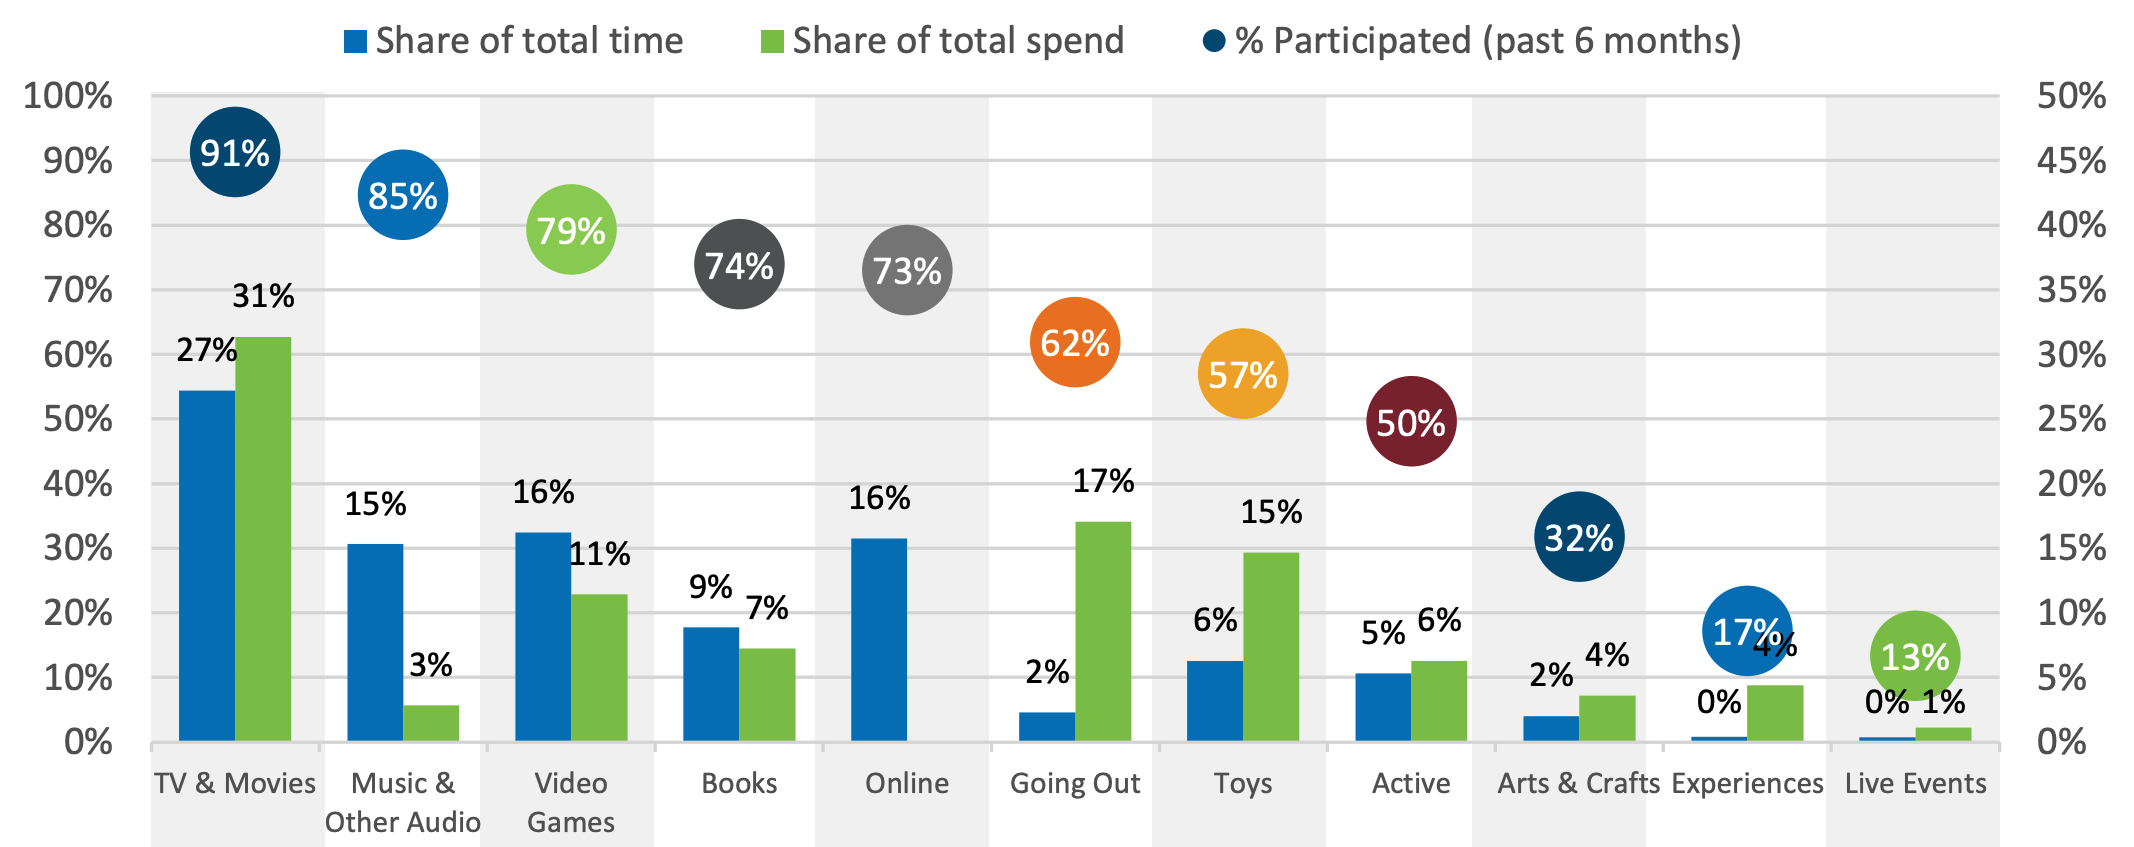
\includegraphics[width=\linewidth]{images/game.png}
    \caption{2020 Report on Entertainment Category Engagement; 79\% of the population is taken by gamers.\\ Source: 2020 Evolution of Entertainment / NPD Group}
    \label{fig:entertainment-report}
\end{figure}

Foldit, designed by researchers at the University of Washington, is a game in which gamers solve protein folding patterns, a central challenge in biochemistry, by virtually wiggling, shaking and pulling shapes to create small stable structures, as well as developing their own algorithms for solving protein folding \cite{bourzac2008enlisting}. This citizen science online game have had more than 800,000 registered players \footnote{As of 13/01/2021, \url{https://fold.it/portal/players}}, identified a potential target for HIV development, and redesigned a catalyst for the Diels-Alder reactions \cite{kreitmair2019citizen}. EyeWire is another example of the success of citizen science gamified environments. With more than 200,00 gamers from 145 countries, EyeWire allows users to map neurons in the retina, filling and extending areas missed by artificial intelligence \cite{kreitmair2019citizen}.

Once focused on ecological and environmental sciences, the citizen science practice has a much larger range now, covering topics such as linguistics \cite{svendsen2018dynamics}, astronomy \cite{marshall2015ideas}, hydrology \cite{buytaert2014citizen} etc. Out of these interest areas, one that could see further development with initiatives using citizen science is Natural Language Processing.

Natural language processing is a vast field that explores how computers can understand and manipulate human language in text or speech format. Researches in this area include (but are not limited to) sentiment analysis, sentence prediction, text translation, text-to-speech conversion, and speech recognition.

Also known as automatic speech recognition (ASR), computer speech recognition, or speech-to-text (STT), speech recognition is a field that studies the recognition and translation of spoken language into text by computers. It has been an intensive research area for decades, but has seen growth led by increased demand on ASR systems in the mobile environment \cite{yu2016automatic}, with virtual assistants, such as Alexa, Siri, Google Now.

Speech recognition is a class of machine learning that has seen many different approaches over time: stochastically modelling with Hidden Markov Models  \cite{gales2008application}, artificial intelligence learning with Neural Networks \cite{graves2013speech}, non-stochastical modelling \cite{burget2003nonrandomattr} and even hybrid approaches \cite{wang2020transformer} have been made to solve this complex interdisciplinary field.

However, these voice modeling strategies are highly dependant on the quality and quantity of data provided. Factors such as noisy speech data, nonhomogeneous recordings, different microphones within the same dataset, and even speech disorders could limit proper analysis, affect accuracy, and even change speech predictions \cite{wrong}. 

These voice datasets, also known as Speech Corpus (or Speech Corpora in plural), curate a collection of audio recordings of a spoken language. Some of them also have additional text files with transcriptions of the words spoken. Although they are widely found in the literature with robust recording procedures and analysis - such as TIMIT \cite{Lamel1992timmit}, DIRHA \cite{Ravanelli2016dirha} and the more recent \cite{chanchaochai2018globaltimit}) -, these datasets are structured in such a way that the speakers are individually selected. This could lead to bias problems \cite{bender2018data}, but also limits the number of voices recorded. Unfortunately, most speech corpora are recorded for the English language \cite{LeRouxVincent2014TRdatasets} and research is limited on the data quantity necessary to enable speech recognition systems and other voice applications.

To circumvent the quantity issue, some corpora are able to be constantly updated with user input. These online datasets can be accessed via web browser. Some examples are Vox Forge and Common Voice \cite{ardila2019common}. However, the former has poor user interface and little usage over time, and the latter has no structured analysis on bias mitigation, relying on crowdsourced information.

This work identifies the Citizen Science practice as a potential candidate to create a robust Speech Corpus for the low-resource Brazilian Portuguese language. A gamifyied application will be constructed to collect the data and engage users, applying data validation techniques to mitigate bias problems afterwards. The curated data will be published in a open-source platform to further research on speech recognition in this low-resource language.

\section*{Objective}

The main focus of this project lies in the construction and validation of a speech corpus for the brazilian portuguese language. The validated corpus and anonymized data will be available to the public.

\chapter{Method}

To achieve the aforementioned objective, this project will:

\begin{itemize}
    \item Research what characterizes a speech corpus in the literature;
    \item Create a list of phrases from which the public will read;
    \item Construct a application to record anonymized speech data;
    \item Add gamification elements to enhance public engagement;
    \item Validate recorded data and apply statistical methods to ensure data quality
    \item Publish dataset on open source platform
\end{itemize}

\section{Document structure}

This document is divided in 4 chapters:

\begin{itemize}
    \item Chapter 1 presents the context, motivation, and objective of the proposed research
    \item Chapter 2 details the background and foundation of all areas related to this research
    \item Chapter 3 presents related work on corpus creation
    \item Chapter 4 presents the systematic literature review to understand what characterizes a speech corpus
    \item Chapter 4 contains the proposed work to finish this research
\end{itemize}

	% ----------------------------------------------------------

% 	% ----------------------------------------------------------
% 	% Metodologia
% 	% ----------------------------------------------------------
	\chapter{Background}
\label{chap:background}

In this chapter, topics such as citizen science, gamification, and speech corpus will be further described. Additional terms relevant to the research will also be defined and clarified, to ensure all research topics are clear. 

\section{Citizen Science}

\subsection{Origins}

The citizen science practice, although not formally defined as so, date back at least a couple of millennia. In ancient China, migratory locusts frequently destroyed harvests, and residents have helped to track outbreaks for some 2,000 years \cite{irwin2018no}. More recently, in 1890, citizen contribution was adopted by the Cooperative Weather Service \cite{quayle1991effects}, where amateurs send collected weather data to the National Weather Service, and continues to provide such data. Later in 1900, the ornithologist Frank Chapman proposed a new holiday tradition - a "Christmas Bird Census" \cite{harden1985christmas}, in which the public would count sighted birds in a predefined area. The Christmas Bird Count contributed to more than 200 publications in the scientific field \cite{kosmala2016assessing}, and the data collected assists the assessment of the health of bird populations, as well as help guide conservation action. In 1966, a similar census started by the North American Breeding Bird Survey contributed to more than 670 publications. The UK Butterfly Monitoring Scheme \cite{pollard1994monitoring}, started in 1976, assess trends in the abundance of butterflies within the United Kingdom, and have supported more than 100 publications.

\subsection{Definition}

The term "Citizen Science" was formally used by Alan Irwin, a sociologist now based at the Copenhagen Business School, with his book "Citizen science: A study of people, expertise and sustainable development" \cite{irwin1995citizen}. Irwin defined citizen science both as “science which assists the needs and concerns of citizens” and as “a form of science developed and enacted by the citizens themselves”. This term was soon modified to describe "a research technique using members of the public to gather or analyze data" \cite{bonney2009citizen}. However, with so many forms of contribution, citizen science now takes a more flexible concept, which can be adapted and applied within diverse situations and disciplines. To encompass this flexibility, the European Citizen Science Association \cite{robinson2018ten} set out some key principles which as a community they believe underlie good practice in citizen science. Appendix \ref{app:ten-principles} lists all ten principles.

\subsection{Classifications}

Below are some classifications in which citizen science projects can be divided:

\subsubsection{Volunteer Involvement}

An initial classification based on volunteer involvement \cite{follett2015analysis}: 
\begin{itemize}
    \item Contributory, where participants contribute to data collection and sometimes help analyze and disseminate results
    \item Collaborative, where citizens also analyze samples, design the study, interpret the data, draw conclusions and disseminate results
    \item Co-created, where they participate in all stages of the project, including defining questions, developing hypotheses, drawing conclusions, discussing results and answering new questions
\end{itemize}

\subsubsection{Goals of the study}

An alternative classification for these initiatives has been suggested by \cite{wiggins2011conservation}, and is based on the goals of the study:

\begin{itemize}
    \item Action projects, initiated by volunteers designed to encourage intervention in local concerns;
    \item Conservation projects, addressing natural resource management goals;
    \item Investigation projects, focusing on scientific research goals in a physical setting;
    \item Virtual projects, also focusing on scientific goals, but entirely based on information technology with all volunteer interaction occurring online;
    \item Education projects; often performed in the classroom or school grounds as part of the science curriculum.
\end{itemize}

\subsubsection{Topic of study}

An additional way of classifying citizen science projects is based on the topic of study, for example, astronomy, archaeology, and biology \cite{wiggins2011conservation}. 

\subsubsection{This work}

If these classifications are to be applied in this work, it should be categorized as a \textbf{contributory virtual speech corpus} citizen science project.

\section{Gamification}

Gamification has been a trending topic as a means of supporting user engagement, being commonly employed in the private sector but also in education, health, government, and science, taking advantage of the widespread activity of game playing \cite{kreitmair2019citizen}. The desire of gamifying services and businesses lies in bringing positive, intrinsically motivating \cite{ryan2000self}, "gamefull" experiences \cite{huotari2012defining} into a service. In the following sections, gamification is (1) defined accordingly to the literature, (2) established through motivational affordances - or game elements, (3) and characterized by some psychological and behavioral outcomes.

\subsection{Definition}

Gamification is commonly defined as "the use of elements of game design in non-game contexts" \cite{deterding2011game}. Although simple, this definition incorporates the succinct method used by gamification. An alternative interpretation by \cite{huotari2012defining} states that gamification is "a process of enhancing a service with affordances for gameful experiences in order to support user's overall value creation". The latter conceptualization suggests the interaction of two actors: (1) the user (using the service) is the creator of value while (2) the service provider can merely provide affordances for the user to experience gamefulness.

\subsection{Motivational affordances (game elements)}

A literature review of empirical studies on gamification by \cite{hamari2014does} defines a list of 10 commonly motivational affordances implemented in table \ref{tab:motivational-affordances}. These 24 peer-reviewed studies were examined, indicating a large variety of different game elements added. The most commonly found were points, leaderboards and badges.

\begin{table}[h]
    \centering
    \caption{Quantity of tested motivational affordances in 24 gamification publications}
    \begin{tabular}{|c|c|}
        \hline Affordance & Publications (out of 24) \\
        \hline Points & 9 \\
        \hline Leaderboard & 10\\ 
        \hline Achievements/Badges & 9 \\
        \hline Levels & 6 \\
        \hline Story/Theme & 6 \\
        \hline Clear goals & 4 \\
        \hline Feedback & 6 \\
        \hline Rewards & 4 \\
        \hline Progress & 4 \\
        \hline Challenge & 7 \\
        \hline
    \end{tabular}
    \caption*{Source: \cite{hamari2014does}}
    \label{tab:motivational-affordances}
\end{table}

\subsection{Psychological and behavioral outcomes}

\subsection{Crowdfunding}

\section{Citizen Science Projects}

With the recent growth of citizen science, various breakthroughs were made possible. Below are some of the most relevant projects in the virtual space, some of which apply gamification to engage contributors.

\subsection{Foldit}

\begin{figure}[ht]
    \centering
    \caption{Foldit - Unfolded (and unstable) Streptococcal Protein Puzzle}
    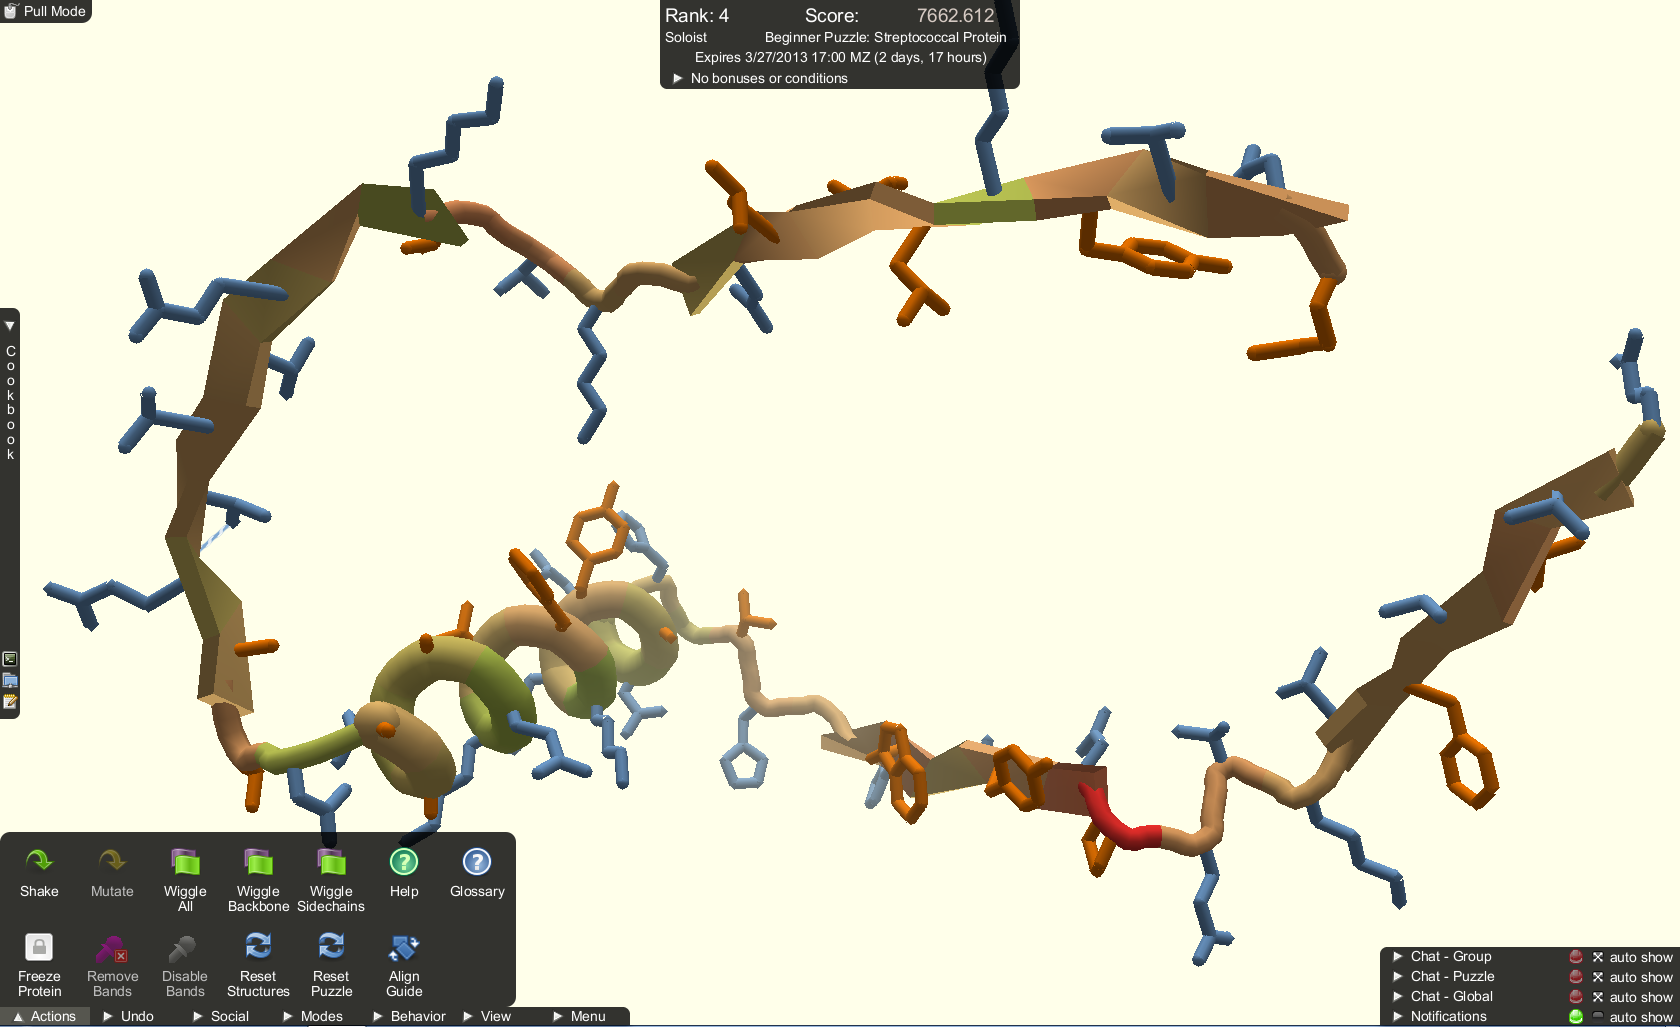
\includegraphics[width=0.8\linewidth]{images/background/foldit-problem.png}
    \caption*{Source: \cite{foldit-protein-problem}}
    \label{fig:foldit-problem}
\end{figure}

Foldit, designed by researchers at the University of Washington, is a game in which gamers solve protein folding patterns, a central challenge in biochemistry, by virtually wiggling, shaking and pulling shapes to create small stable structures, as well as developing their own algorithms for solving protein folding \cite{bourzac2008enlisting}. 

\begin{figure}[ht]
    \centering
    \caption{Foldit - Folded up Streptococcal Protein Puzzle}
    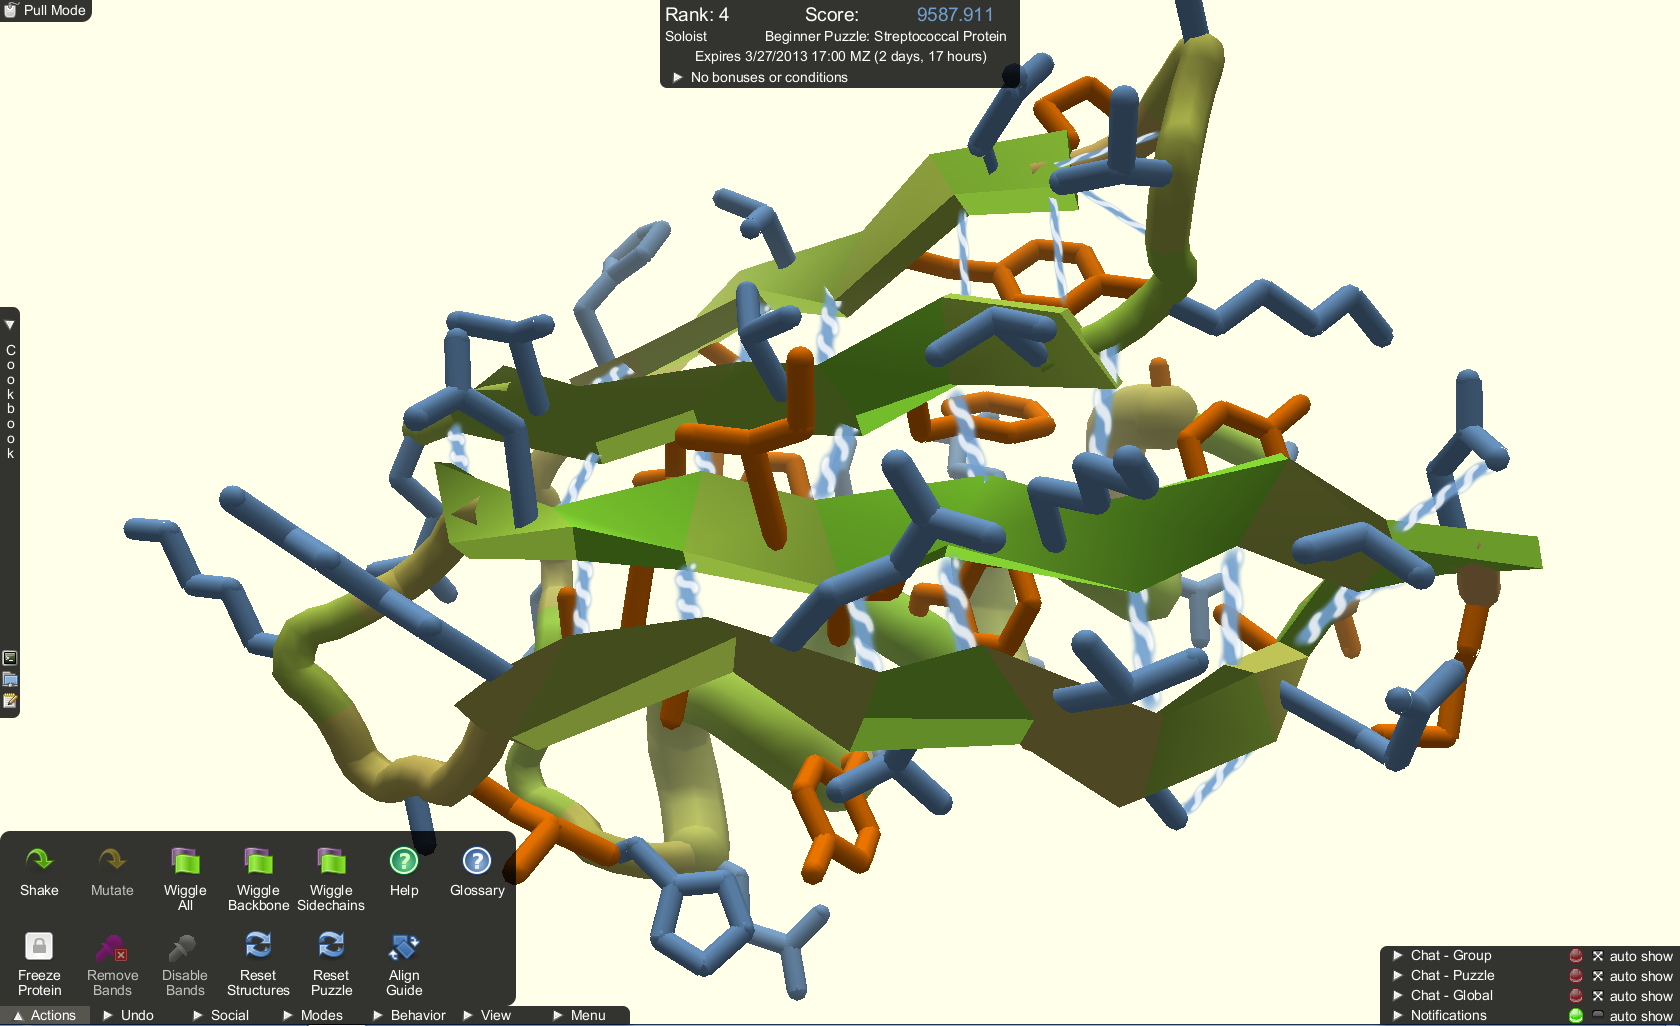
\includegraphics[width=0.8\linewidth]{images/background/foldit-solution.png}
    \caption*{Source: \cite{foldit-protein-solution}}
    \label{fig:foldit-solution}
\end{figure}

As the moment of this article, Foldit has had 20 peer-reviewed articles in a number of journals and conferences \cite{foldit2021publications}. Some relevant breakthroughs are a potential target for HIV drug development \cite{khatib2011crystal}, redesign of the catalyst for the Diels-Alder reaction \cite{eiben2012increased}, and improvement of cryo-electron microscopy atomic model building and refinement \cite{khatib2019building}.

\subsubsection{Gamification in Foldit}

To appeal to the general public, Foldit applies gamification in many different elements. The main objective of the game is to obtain the most stable and folded protein. To encourage this optimization, the user interface assigns a score to the protein, relative to how well it is folded. The best solutions to these puzzles are displayed in a ranking system, to promote competition between users. Another element to aid engagement is social. Users create and join groups, and members of groups can share puzzle solutions. These groups have been found to be useful in training new players.

\subsection{EyeWire}

\begin{figure}[ht]
    \centering
    \caption{EyeWire game interface}
    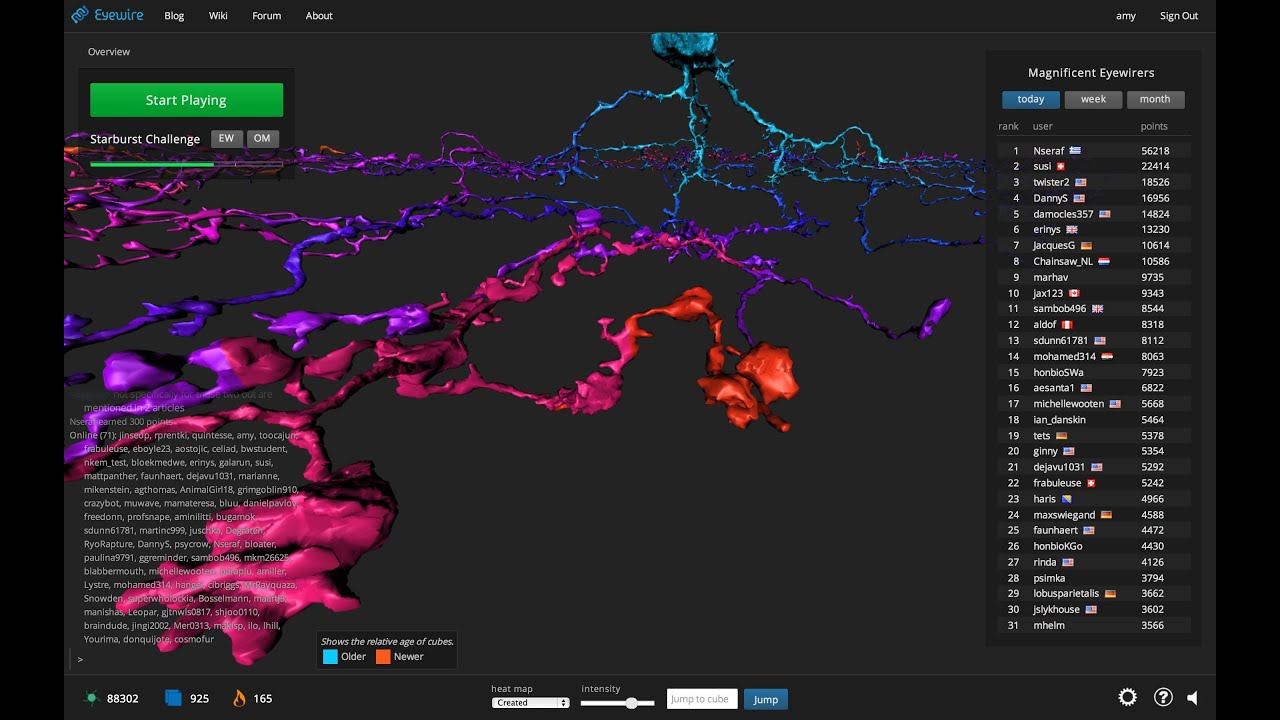
\includegraphics[width=0.8\linewidth]{images/background/eyewire.jpg}
    \caption*{Source: \cite{eyewire2014how}}
    \label{fig:eyewire-game-interface}
\end{figure}

EyeWire is a Web-based citizen science game that aims to create a detailed atlas of the human brain. Nonprofessionals are asked to map connections of neurons which reside in the back of the human eye. This mapping is done through 3D-transformed functional magnetic resonance images (fMRI), and combines crowd contributions with machine learning algorithms to help neuroscientists to achieve a better understanding of visual stimuli processing by humans.

\subsubsection{Gamification in EyeWire}

EyeWire transforms the complex task of brain mapping into smaller (micro) tasks via a gaming interface with several elements associated \cite{seaborn2015gamification}. This has been identified as a positive motivation for a player's participation \cite{tinati2016because}. Other elements such as music, sound effects, interactive tutorials, leaderboard, and a chat interface add to the overall experience, creating a fun experience. According to a survey on EyeWire motivation \cite{tinati2016because}, 57\% out of 349 respondents considered the the game entertaining.

\subsection{Galaxy Zoo}

\begin{figure}[ht]
    \centering
    \caption{Hubble's Galaxy Classification Schema to help new players classify galaxies}
    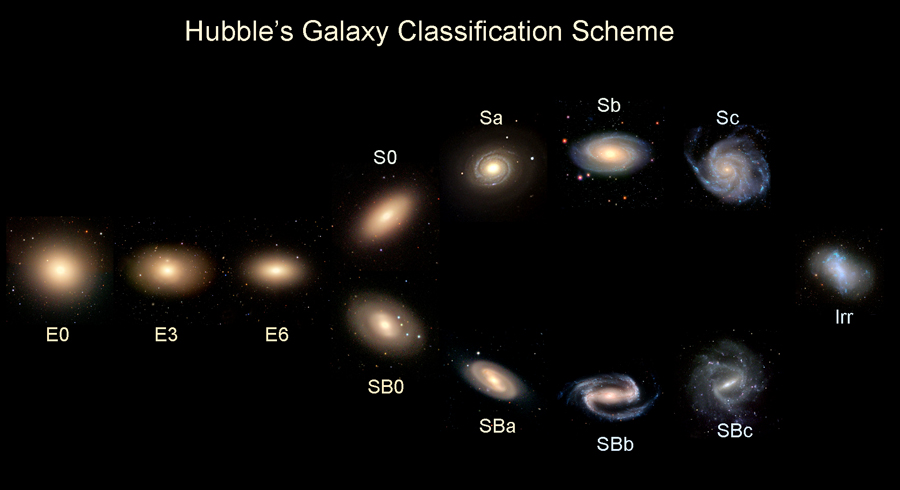
\includegraphics[width=0.8\linewidth]{images/background/galaxyzoo-training.jpg}
    \caption*{Source: \cite{galaxyzoo2010hubble}}
    \label{fig:galaxyzoo-hubble}
\end{figure}

In July 2007, Galaxy Zoo was a simple online citizen science initiative that asked volunteers to morphologically classify selected images of galaxies by the Sloan Digital Sky Survey (\cite{york2000sloan} executed at Apache Point Observatory by the SDSS 2.5m telescope). In this first iteration, Galaxy Zoo has had more than 100,000 volunteers classifying nearly 900,000 galaxies \cite{lintott2011galaxy}. The unexpected popularity has inspired the creation of Zooniverse, hosting project using the same technique across many research areas \cite{zooniverse2021galaxy}.

After its end in 2009, Galaxy Zoo was followed by Galaxy Zoo 2 (GZ2). The second incarnation extends the original Galaxy Zoo classifications for a subset of the brightest galaxies in the legacy release, measuring more detailed morphological features. This iteration contributed to 60 million classifications on more than 250,00 SDSS galaxies by more than 80,000 volunteers \cite{galaxyzoo22021volunteers}.

Including the latest issue of Galaxy Zoo (started in 2018), the initiative has supported the publication of 82 articles \cite{galaxyzoo2021publications}, helping analyze elements such as: galaxy rotation, color of elliptical galaxies, galaxy dust, galaxy bulges, etc.

\subsubsection{Gamification in Galaxy Zoo}

Galaxy Zoo utilizes the Zooniverse platform for data classification. This platform is not a gamified environment, thus relying on other forms of engagement to retain users, such as interest in astronomy, enjoyment of looking at galaxy pictures, desire and excitement to contribute to scientific research, etc \cite{raddick2009galaxy}.

\subsection{Zooniverse}

\begin{figure}[ht]
    \centering
    \caption{Zooniverse Platform, connecting volunteers with scientists}
    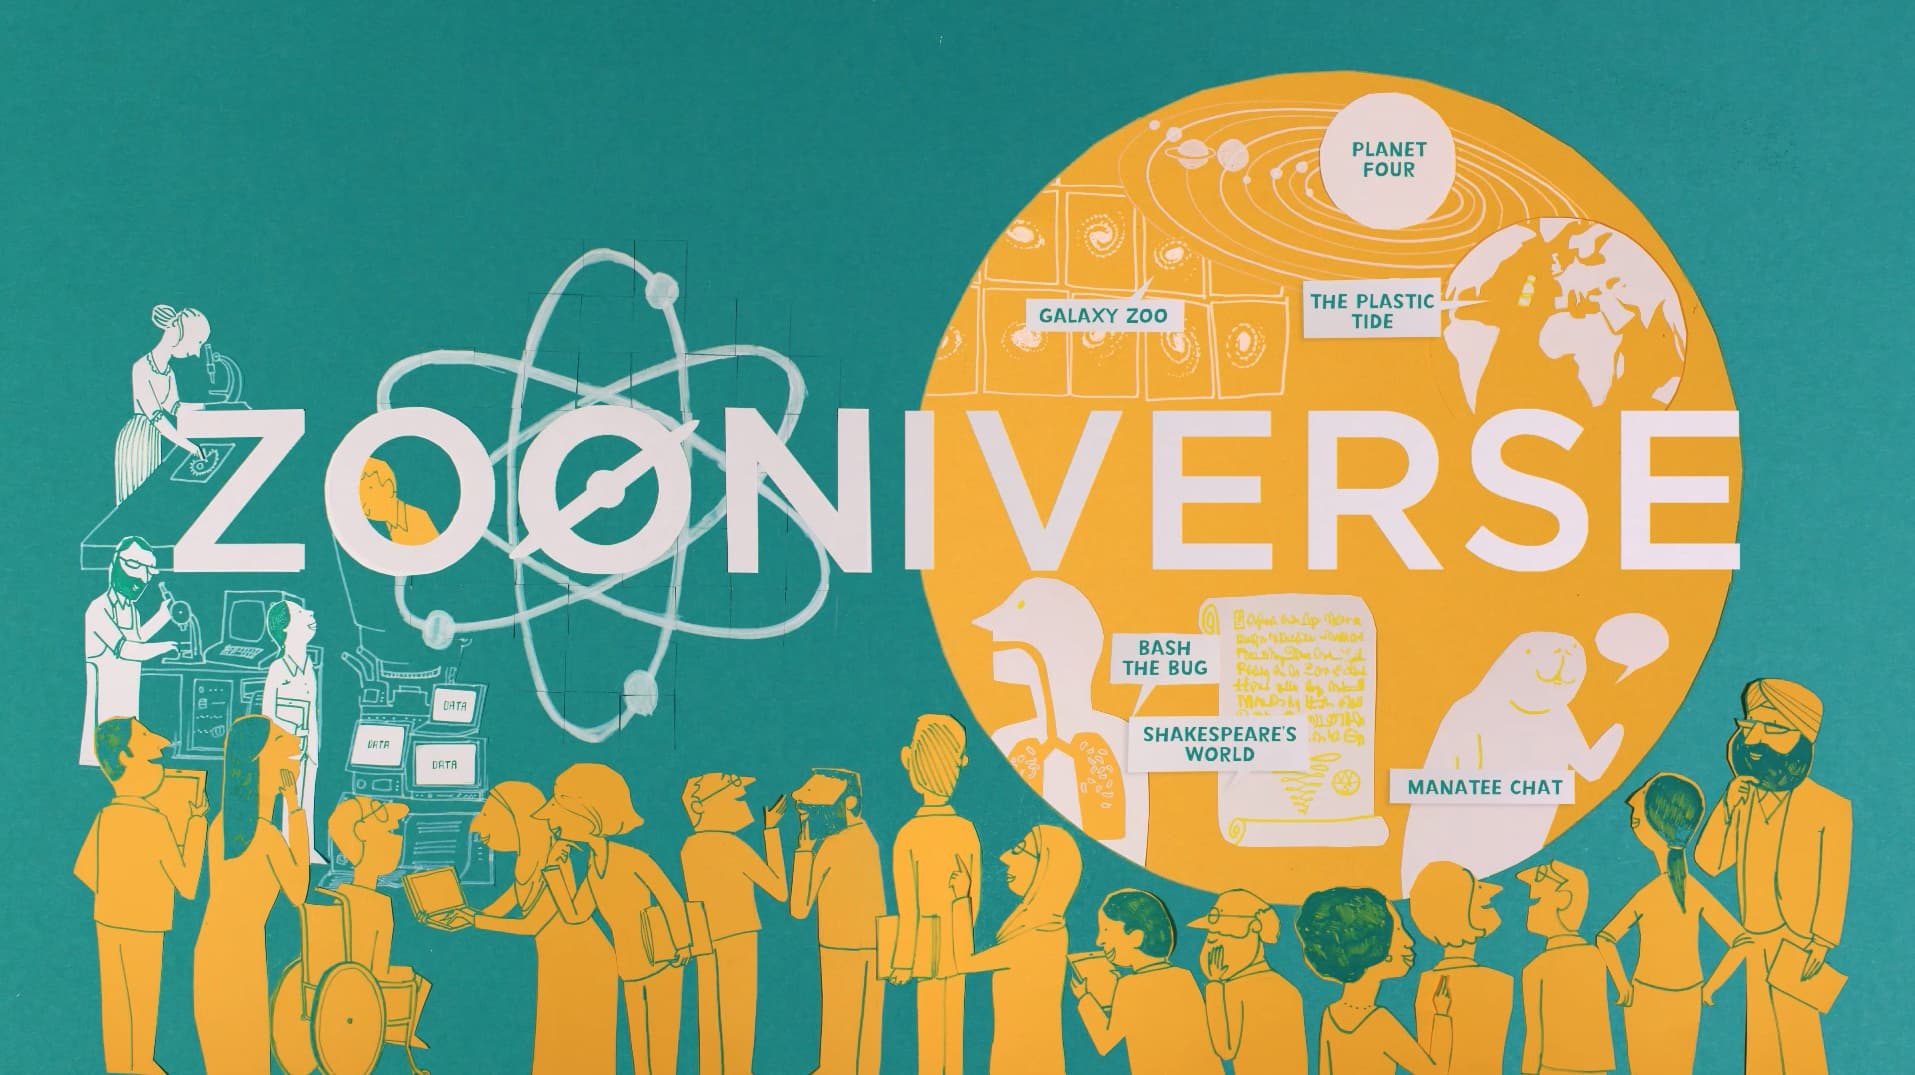
\includegraphics[width=0.7\linewidth]{images/background/zooniverse.jpg}
    \caption*{Source: \cite{zooniverse-logo}}
    \label{fig:foldit-solution}
\end{figure}

Zooniverse is a platform for citizen science projects. It connects more than a million volunteers around the world to assist professional researchers. The platform has a simple interface for input and classification of data, as well as the creation and management of projects.

This collaborative platform has enabled over 300 of scientific publications, with publications on the discovery and classification of stars, planets, supernovas; humanities, animal identification, classification of whale calls, datasets, etc. The following projects started in Zooniverse and each have their own characteristics:

\subsection{Penguin Watch}

\begin{figure}[ht]
    \centering
    \caption{Penguin Watch interface - Penguins are marked as adults and chicks}
    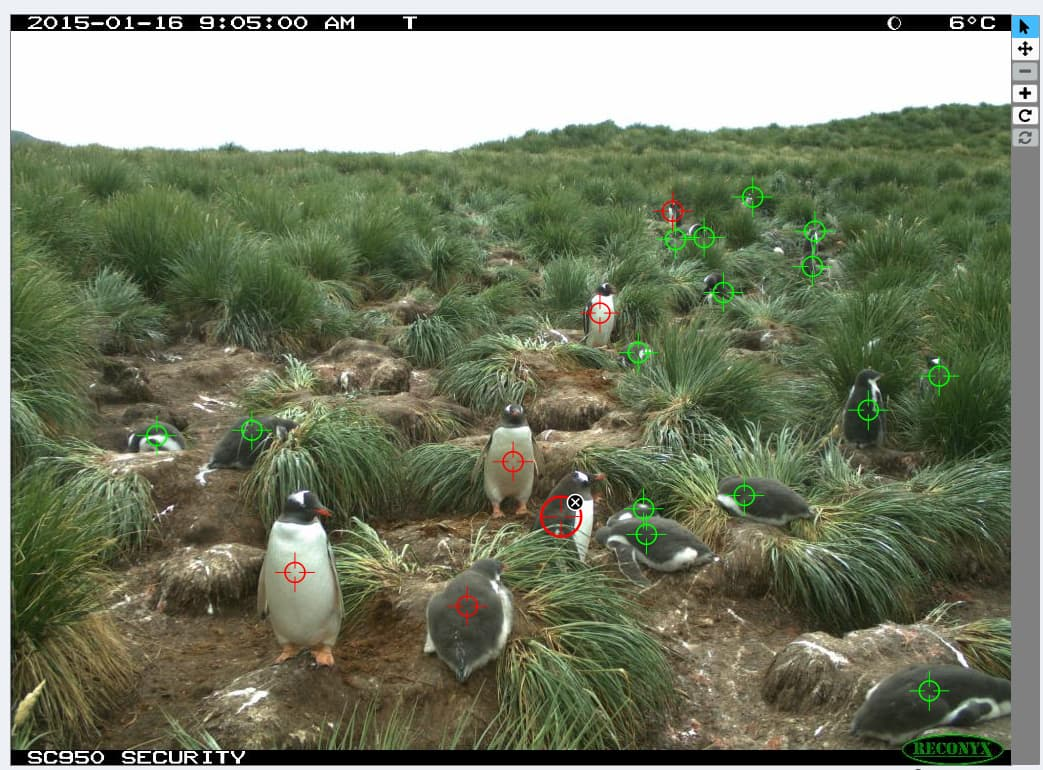
\includegraphics[width=0.8\linewidth]{images/background/penguinwatch.jpg}
    \caption*{Source: \cite{penguin2015watch}}
    \label{fig:oldweather-logbook}
\end{figure}

The Penguin Watch citizen science project states that by monitoring the population change in seabirds like penguins, it is possible to identify changes occurring in the wider ecosystem. These changes can help create health indicators of the marine environment, but the lack of the ability to collect and analyze such amounts of data made a team of researchers create the Penguin Watch initiative. Contributors help identify penguins in images of various sites over the world by using a web interface in Zooniverse.

\subsubsection{Gamification in Penguin Watch}

Like with GalaxyZoo, Penguin Watch runs their contribution platform over Zooniverse. While the platform does take responsibility in maintaining infrastructure and service management, it does not include gamification elements in the classification interface.

\subsection{Contributions}

The table \ref{tab:cs-contributions} contains an aggregated list of contributors and contributions from the projects described above.

\begin{table}[h]
\centering
\begin{threeparttable}
    \caption{Contribution for online citizen science projects}
    \small{
    \begin{tabular}{|c|c|c|}
        \hline 
        Project & Contributors & Publications \\ \hline
        Foldit & 855,350 \cite{foldit2021players} & 20 \cite{foldit2021publications} \\ \hline
        EyeWire & 300,000 \cite{eyewire2017players} & 3 \cite{eyewire2021publications} \\ \hline
        Penguin Watch & 28,500 \cite{penguin2021players} & 10 \cite{penguin2021publications} \\ \hline
        Galaxy Zoo (2007-2009) & 100,000+ \cite{lintott2011galaxy} & \multirow{3}{*}{82 \cite{galaxyzoo2021publications}\tnote{~a}} \\ \cline{1-2} 
        Galaxy Zoo 2 (2009-2013) & 80,000+ \cite{galaxyzoo22021volunteers} & \\ \cline{1-2} 
        Galaxy Zoo (2018-2021) & 61,149 \cite{galaxyzoo2021players} & \\ \hline 
    \end{tabular}}
    \begin{tablenotes}
        \item[a] Across all Galaxy Zoo Iterations, including Radio and Supernova Galaxy Zoo.
    \end{tablenotes}
\end{threeparttable}
\caption*{Source: Author}
\label{tab:cs-contributions}
\end{table}

\section{Natural Language Processing}

\subsection{Speech Recognition}

\section{Speech Corpus}

\section{Noisy data}

A common issue with these croudsourced online datasets lies in data quality. Disparities in recorded noise, environment change, recording length variation, and general quality of the recording are intrinsically associated with these contributions, since volunteers have each their own devices and recording conditions. To mitigate these issues, work has been made in the post-processing of these recordings \cite{krishna2019speech}.

\section{Licencing}
\subsection{GPL}
\subsection{CC0}

\section{Systematic Literature Review}


	\chapter[Related Work]{Related Work}

In this section, we discuss how the literature has treated speech corpora creation, as well as the various conditions and variables considered in the process. Speech Corpus crafting itself is well established in the literature by TIMIT \cite{Lamel1992timmit} and SWITCHBOARD \cite{godfrey1992switchboard}. TIMIT creates a dataset of 6300 utterances by 630 speakers from different regions of the United States. The sentences were crafted to fit in one of the three categories: 1) dialect "shibboleth", 2) phonemically compact and 3) phonetically diverse, but the selection itself was not well defined. Nevertheless, it is a very robust dataset with a time-aligned transcription and a usage guide to automatic speech recognition applications.

The CHiME articles \cite{christensen2010chime} \cite{barker2013pascal}, \cite{barker2018fifth} (and more), are also source of structured speech corpora creation, challenging researchers to better recognize speech within a everyday listening environment using multiple distant microphones. Since the focus of these works lies on nonoptimal recording conditions, detailed information on the noise background, noise level, recording style and speech material has been provided, as well as comprehensive postprocessing work.

A more recent work by \cite{chanchaochai2018globaltimit} attempts to extend the TIMIT functionality to other languages, by providing a method to create "TIMIT-like" datasets. These datasets are caracterized by having 1) Multiple (anonymously) identified speakers, 2) Wide range of phonetically representative inputs, 3) Wideband recordings with good acoustic quality, 4) Time-aligned lexical and phonemic transcripts and 5) Easily availability to anyone. The authors detail the speakers and sessions, the text corpus selection process, the recording procedures, as well as the transcription and alignment methods. At the moment, there have been five datasets created, with more planned or in progress.

	\chapter{Systematic Literature Review}
\label{chap:slr}

To identify the characteristics of a speech corpus, a systematic literature was performed \cite{kitchenham2009systematic}.

The search was executed on August 1st, 2019 and the electronic database used was Web of Science. Since corpora are also presented at conferences, all article types were considered in the search, not limited by publication date. The whole process to choose relevant papers is defined below:

\section{Search in papers database}

The first step in the process is searching for papers in the specified database. To allow reproducibility, the search query is presented in table \ref{tab:search-terms}. No criteria were applied in the search, therefore considering the title, abstract, keywords, and the entire paper for indexing. It is also noted that conference proceedings are also included in this search. In this step, 157 results were yielded. This result was further filtered to 23, which contained the terms in the title.

\begin{table}[h]
    \centering
    \caption{Search terms used in the SLR}
    \begin{tabular}{|c|c|}
        \hline Digital Library & Search terms \\ \hline
        Web of Science & TOPIC: ("speech corpus" OR "speech corpora")  \\ \hline
    \end{tabular}
    \caption*{Source: Author}
    \label{tab:search-terms}
\end{table}

\section{Inclusions and exclusions}

To filter relevant results, we define the criteria to include or exclude the articles based on each abstract read:

\subsection{Inclusion Criteria}

\begin{itemize}
    \item Creates a speech corpus
    \item Define or discuss speech corpus creation
\end{itemize}

\subsection{Exclusion Criteria}

\begin{itemize}
    \item Full text not available in the electronic document
    \item Does not contain "speech corpus" or "speech corpora" strings in title, abstract, or keywords.
\end{itemize}

This step reduced the number of articles to 14.

\section{Article Analysis}

After applying the proper filtering as defined in the previous section, the remaining articles can be fully read to find the results. The whole filtering process is summarized in \ref{tab:filtering}.

\begin{table}[h]
    \centering
    \caption{SLR - Filtering of results}
    \begin{tabular}{|c|c|}
        \hline Step & Results \\ \hline
        Initial search & 157 \\ \hline
        Title filtering & 23 \\ \hline
        Abstract reading & 14 \\ \hline
    \end{tabular}
    \caption*{Source: Author}
    \label{tab:filtering}
\end{table}

\section{Findings}

To analytically organize our findings, a content-analysis approach was used. To choose the categories in which the content analysis is applied, we adapted the work from \cite{queiroz2019blockchain}, resulting in table \ref{tab:content-analysis}. As for the corpus categories, we sought a comparison work from  \cite{LeRouxVincent2014TRdatasets}, in which a comprehensive table was provided and adapted to fit our categorization needs.

\begin{table}[h]
    \centering
    \caption{Categories for content analysis}
    \begin{tabular}{|p{4cm}|p{11cm}|}
        \hline Category & Explanation/Example \\ \hline
        Total number of papers published & Number of publications by year \\ \hline
        Application area & Speech Corpus, Learning English Pronunciation, Automatic Speech Recognition, Crowdsourcing \\ \hline
        Application context & Speech Corpus Creation, Speech Corpus Automated Analysis, Dialect Analysis \\ \hline
        Corpus Language & English (Dialect), Arabic, Multilingual, etc \\ \hline
    \end{tabular}
    \caption*{Source: Author}
    \label{tab:content-analysis}
\end{table}

\begin{table}[h]
    \centering
    \caption{Categories for speech corpus construction}
    \begin{tabular}{|p{4cm}|p{11cm}|}
        \hline Category & Explanation/Example \\ \hline
        General attributes & scenario, total duration, sampling rate, number of distant or noisy microphones, demographics, transcription and time alignment and open access \\ \hline
        Speech attributes & duration of speech, speaking style, speakers in the room, speaker overlap\\ \hline
        Channel attributes & channel type, speaker location, speaker movements \\ \hline
        Noise attributes & stationary background noise, car noise, meeting noises, domestic noises, outdoor noises \\ \hline
        Available ground truth & reference speech signal, speaker location and orientation, paralinguistic attributes, noise events \\ \hline
    \end{tabular}
    \caption*{Source: Author}
    \label{tab:speech-analysis}
\end{table}

\subsection{Publication by country and year}

Table \ref{tab:country-analysis} reports the number of papers, published by country and year, resulting from the research protocol application.

\begin{table}[h]
    \centering
    \caption{Countries for content analysis}
    \begin{tabular}{|c|c|c|c|c|c|}
        \hline Country & 2005-2015 & 2016 & 2017 & 2018 & (\%) \\ \hline
        United States & - & 3 & 2 & - & 33\% \\ \hline 
        Japan & 3 & - & - & - & 20\% \\ \hline
        Emirates Arabs & - & - & 1 & 1 & 13\% \\ \hline
        India & - & - & 1 & - & 6.7\% \\ \hline
        Malasya & - & - & 1 & - & 6.7\% \\ \hline
        Sweden & - & - & 1 & - & 6.7\% \\ \hline
        China & - & 1 & - & - & 6.7\% \\ \hline
        Poland & 1 & - & - & - & 6.7\% \\ \hline
    \end{tabular}
    \caption*{Source: Author}
    \label{tab:country-analysis}
\end{table}

\subsection{Publication by type}

As for publication types, they have almost been equally divided: 46.7\% for articles and 53.3\% for proceedings papers.

\subsection{Speech Corpus studies' categorization}

In table \ref{tab:results-categorization}, each article is categorized according to table \ref{tab:content-analysis} definitions. The analysis is done afterwards in section \ref{sec:discussion}.

\begin{landscape}
\begin{longtable}{|p{2cm}|p{4.5cm}|p{10cm}|p{4.5cm}|}
\caption{Findings organized by speech corpus categorization as per table \ref{tab:content-analysis}}
\label{tab:results-categorization}
    \hline Authors & Application area & Context & Language \\ \hline
    \cite{almeman2018building} & Read Corpus & Multi-dialect Arabic corpora is scarce and not generated on mobile & Arabic \\ \hline
    \cite{dwivedi2017documenting} & Language Documentation & Revitalization of endangered languages through corpus creation & Kanauji of Kanpur \\ \hline
    \cite{bougrine2017altruistic} & Crowdsourcing & Crowdsourcing is a emerging and collaborative approach and can be effectively used to annotate linguistic resources & Arabic Algerian Dialects \\ \hline
    \cite{ng2017shefce} & Automatic syllable and phoneme detection & Pronunciation assessment studies in a bilingual context & Billingual (Cantonese, English) \\ \hline
    \cite{moore2017sheffield} & Read Speech & Goal oriented conversation & British English with a southern accent \\ \hline
    \cite{ramli2017first} & Storytelling Speech & Under-resourced language corpus creation for humanoid robot storyteller & Malay \\ \hline
    \cite{mansikkaniemi2017automatic} & Automatic speech alignment & Transcribed speech is a scarce and expensive resource & Finish \\ \hline
    \cite{goldman2016siwis} & Cross language speaker adaptation & Cross-lingual studies have no speech corpus from the same speakers & Bilingual and Trilingual from (English, French, German and Italian) \\ \hline
    \cite{liu2016sheffield} & Spontaneous Speech & Distant speech recognition with multi-channel speech corpus & English \\ \hline
    \cite{ruilan2016improving} & Read Corpus & Pronunciation characteristics in non-native English speakers & Dialectal English \\ \hline
    \cite{klessa2013paralingua} & Read Corpus & Paralinguistic features detection for forensics & Paralinguistic \\ \hline
    \cite{nagino2008building} & Corpus Enhancement & Low cost speech corpus creation with statistical multidimensional scaling method & Japanese \\ \hline
    \cite{zhang2008improved} & Phonetic words selection & Phonetically rich word selection from larger corpus & Chinese \\ \hline
    \cite{clopper2006nationwide} & Read Corpus & Large amount of speech by male and female from six dialect regions & Multiple-dialect English \\ \hline
\caption*{Source: Author}
\end{longtable}
\end{landscape}

\begin{landscape}

\begin{table*}[h]
\centering
\caption{Speech corpora characteristics defined in table \ref{tab:speech-analysis}}
\begin{tabular}{|p{4cm}|p{5cm}|p{7cm}|p{3.5cm}|}
\hline
Category & Characteristic & Work(s) & Quantity (out of 14)  \\ \hline
\multirow{7}{*}{General attributes} 
    & Scenario & 
    \cite{almeman2018building}, \cite{dwivedi2017documenting}, \cite{bougrine2017altruistic}, \cite{bougrine2017altruistic}, \cite{moore2017sheffield}, \cite{ramli2017first}, \cite{goldman2016siwis}, \cite{liu2016sheffield}, \cite{ruilan2016improving}, \cite{klessa2013paralingua}, \cite{nagino2008building},  \cite{clopper2006nationwide}, \cite{zhang2008improved} & 13
    \\ \cline{2-4} & Total duration &
    \cite{dwivedi2017documenting}, \cite{bougrine2017altruistic}, \cite{bougrine2017altruistic}, \cite{moore2017sheffield}, \cite{ramli2017first}, \cite{goldman2016siwis}, \cite{liu2016sheffield}, \cite{ruilan2016improving}, \cite{klessa2013paralingua}, \cite{nagino2008building}, \cite{clopper2006nationwide}, \cite{zhang2008improved} & 12
    \\ \cline{2-4} & Sampling Rate &
    \cite{almeman2018building}, \cite{dwivedi2017documenting}, \cite{bougrine2017altruistic}, \cite{ng2017shefce}, \cite{moore2017sheffield}, \cite{ramli2017first}, \cite{goldman2016siwis}, \cite{liu2016sheffield}, \cite{ruilan2016improving}, \cite{klessa2013paralingua}, \cite{clopper2006nationwide} & 11
    \\ \cline{2-4}& Distant or noisy microphones & 
    \cite{moore2017sheffield}, \cite{ramli2017first}, \cite{liu2016sheffield} & 3
    \\ \cline{2-4} & Demographics &
    \cite{dwivedi2017documenting}, \cite{bougrine2017altruistic}, \cite{ng2017shefce}, \cite{goldman2016siwis}, \cite{ruilan2016improving}, \cite{klessa2013paralingua}, \cite{clopper2006nationwide} & 7
    \\ \cline{2-4} & Transcription and time alignment & % manual?
    \cite{dwivedi2017documenting}, \cite{bougrine2017altruistic}, \cite{bougrine2017altruistic}, \cite{ng2017shefce}, \cite{moore2017sheffield}, \cite{ramli2017first}, \cite{goldman2016siwis}, \cite{liu2016sheffield}, \cite{ruilan2016improving}, \cite{klessa2013paralingua}, \cite{nagino2008building}, \cite{clopper2006nationwide} & 12
    \\ \cline{2-4} & Open access &
    \cite{almeman2018building}, \cite{moore2017sheffield}, \cite{liu2016sheffield} & 3
\\ \hline \multirow{3}{*}{Speech attributes}
    & Unique words & 
    \cite{bougrine2017altruistic}, \cite{bougrine2017altruistic}, \cite{ng2017shefce}, \cite{moore2017sheffield}, \cite{ramli2017first}, \cite{goldman2016siwis}, \cite{liu2016sheffield}, \cite{ruilan2016improving}, \cite{klessa2013paralingua}, \cite{nagino2008building}, \cite{clopper2006nationwide} & 11
    \\ \cline{2-4} & Speaking style &
    \cite{dwivedi2017documenting}, \cite{bougrine2017altruistic}, \cite{ng2017shefce}, \cite{moore2017sheffield}, \cite{ramli2017first}, \cite{goldman2016siwis}, \cite{nagino2008building}, \cite{clopper2006nationwide} & 8
    \\ \cline{2-4} & Number of speakers & 
    \cite{dwivedi2017documenting}, \cite{bougrine2017altruistic}, \cite{bougrine2017altruistic}, \cite{ng2017shefce}, \cite{moore2017sheffield}, \cite{ramli2017first}, \cite{goldman2016siwis},, \cite{ruilan2016improving} \cite{liu2016sheffield}, \cite{klessa2013paralingua}, \cite{nagino2008building}, \cite{clopper2006nationwide} & 14
\\ \hline \multirow{3}{*}{Channel attributes}
    & Channel type & 
    \cite{dwivedi2017documenting}, \cite{bougrine2017altruistic}, \cite{ng2017shefce}, \cite{moore2017sheffield}, \cite{ramli2017first}, \cite{goldman2016siwis}, \cite{liu2016sheffield}, \cite{ruilan2016improving}, \cite{nagino2008building}, \cite{clopper2006nationwide} & 10
    \\ \cline{2-4} & Speaker location & 
    \cite{dwivedi2017documenting}, \cite{ng2017shefce}, \cite{liu2016sheffield} & 3
    \\ \cline{2-4} & Speaker movements & 
    \cite{dwivedi2017documenting}, \cite{moore2017sheffield}, \cite{liu2016sheffield} & 3
\\ \hline \multirow{1}{*}{Noise attributes}
    & Noise type & N/A &
    0
\\ \hline \multirow{4}{*}{Available ground truth} 
    & Reference speech signal & 
    \cite{ng2017shefce}, \cite{moore2017sheffield}, \cite{ramli2017first}, \cite{liu2016sheffield} & 4
    \\ \cline{2-4} & Speaker location and orientation &
    \cite{bougrine2017altruistic}, \cite{moore2017sheffield}, \cite{ramli2017first}, \cite{liu2016sheffield} & 4
    \\ \cline{2-4} & Paralinguistic attributes &
    \cite{klessa2013paralingua} & 1
    \\ \cline{2-4} & Noise events & 
    \cite{ramli2017first} & 1
    \\ \hline
\end{tabular}
\caption*{Source: Author}
\label{tab:results-attributes}
\end{table*}
\end{landscape}

\section{Discussion}
\label{sec:discussion}

Each of our findings is discussed in the following subsections.

\subsection{Publications by country and year}

A simple analysis on table \ref{tab:country-analysis} infers that the research on speech corpus creation was stable until 2018, which had its last article published. This can be explained by the limited number of "Open Access" articles found and the small number of databases searched (Web Of Science only). A more permissive literature review should be able to better understand the conditions on which non-open articles are being released, as well as enhance coverage of the state-of-the-art in this field.

The table also categorizes the countries research quota. More developed countries such as United States and Japan have created more corpora over the years.

\subsection{Publications by type}

In the search executed, the remaining articles were almost equally separated by type. A great number of conference proceedings may indicate that the corpus creation process is not properly defined, as works vary in content and structure. Again, the main limitation of this work is the only database searched, therefore skewing analysis.

\subsection{Speech corpus categorization}

Table \ref{tab:content-analysis} contains the content-analysis for the works in the systematic literature review. Two of the columns - Application Area (1), and Language (2) - are be discussed below:

\subsubsection{Application Area}

Most of the corpora found in the articles were a Read Speech Corpus (\cite{almeman2018building}, \cite{ruilan2016improving}, \cite{klessa2013paralingua}, \cite{clopper2006nationwide}), revealing the lack of structured language documentation in the current research. This can be explained by the type of its content: a scripted content, with less bias from the speakers when compared to spontaneous corpora. Three of these works (\cite{ng2017shefce}, \cite{mansikkaniemi2017automatic} and \cite{nagino2008building}) worked on automating corpus creation by automatically aligning words, detecting syllables and phonemes, and even enhancing corpora, as currently most recording and alignment work is done manually.

\subsubsection{Languages}

There is a significant number of dialect and multilingual corpora research in the analyzed works. These variations of the same language - in different regions, or by different pronunciation by non-native speakers -, suggest that speech technology could become more personalized as computers understand less traditional utterances of the same language.

\subsection{Works by speech corpus characteristics}

Our findings condensed in table \ref{tab:results-categorization} illustrate the
current speech corpus creation characteristics used in the literature, each discussed below:

\subsubsection{Scenario}

Almost all corpora specified the scenario at which the recordings were executed. A meeting room (\cite{liu2016sheffield}, \cite{moore2017sheffield}); a anechoic booth (\cite{goldman2016siwis}); a quiet room inside a laboratory (\cite{ramli2017first}), etc. Although, each corpus is not limited to one scenario. For instance, \cite{almeman2018building} recorded in four different scenarios: inside the home, in a moving car, in a public place, and in a quiet place. Such characteristic is critical to corpus creation.

\subsubsection{Total duration}

12 out of the 14 studies analyzed described the total duration of the recordings. This illustrates the importance of being descriptive in the corpus.

\subsubsection{Sampling Rate}

The sampling rate is major to the corpus creation. It is cited in 11 out of the 14 works read. The reason it has so much importance lies on the corpus main usage: automatic speech recognition software. Knowing the frequency at which the recordings are done, the computer is able to better recognize subtleties in a more sampled audio, as well as simplify processing in a lower frequency sample rate.

\subsubsection{Noisy microphones}

Non-optimal recording conditions are normal. For instance, speaking on the phone in a public space generates a very high noisy background \cite{moore2017sheffield}). Moreover, speaking far from the microphone is also a common occurrence. The presence of works in this category emphasizes the need of noisy corpora to ensure automatic speech recognition software takes these factors into account.

\subsubsection{Demographics}

When recording accent (\cite{moore2017sheffield}), dialect (\cite{almeman2018building}) and pronunciation (\cite{ng2017shefce}), the definition of speaker demographics supports the understanding of the variations between the same language through research.

\subsubsection{Transcription and time alignment}

In the context of automatic speech recognition, a speech corpus containing  transcription and time alignment (additional to the recordings) enable computers and speech recognition specialists a more faithful analysis. Its importance can be verified by 85\% of the works evaluated.

%\subsubsection{Open access}

%Most corpora are closed to the public viewer. 

%\subsubsection{Unique words}
%\subsubsection{Speaking style}
\subsubsection{Number of speakers}

As well as the total duration, the number of speakers is a major characteristic of the corpus. More speakers lead to more representativeness, but also affect the corpus recording time. It is an important parameter and every paper analyzed describes it.

	\chapter[Proposal]{Proposal}

This proposal focuses on detailing the necessary steps to the creation and publication of a crowdfunding speech corpus in Brazilian Portuguese. To this end, a virtual voice recording application will be developed (section \ref{sec:proposal-app}), focusing on adding gamification elements to enhance user engagement. Additionally, this application will also extract some relevant characteristics found in the systematic literature review in chapter \ref{chap:slr}. Once the construction is finished, the application will be released, allowing general public submission (in section \ref{sec:proposal-public-submission}). After the submission period, the collected data will be analyzed and compiled to a speech corpus (\ref{sec:proposal-data-analysis}), which will be publicized to an open-source repository in section \ref{sec:proposal-data-publication}.

\section{Application}
\label{sec:proposal-app}

This section details the conception, documentation, and development process of the voice recording application, coined "Fale Alguma Coisa". Below, it will at times be referenced as "app", short for application.

\begin{figure}[ht]
    \centering
    \caption{Fale Alguma Coisa app Logo}
    
\includegraphics[width=\linewidth/2]{images/app/logo.jpg}
    \caption*{Source: Author}
    \label{fig:falealgumacoisa-logo}
\end{figure}

\subsection{Concept}

The Fale Alguma Coisa app should provide an easy gateway for you to contribute your voice while having fun and learning various science facts and curiosities.

\subsection{Target Audience}

Directed towards anyone interested in learning and contributing to science.

\subsection{User Stories}

The development of most software starts with its documentation. This work chose a user story approach to project documentation and lists them below, categorized by epic.

\subsubsection{Usability}

\begin{itemize}
    \item I, as a citizen, would like to contribute my voice using my mobile devices and desktop computer.
\end{itemize}

\subsubsection{Homepage}

The homepage epic represents the user stories affecting the homepage, such as the splash screen, call to action button, terms of service, etc.

\begin{itemize}
    \item I, as an unregistered citizen, would like to view an animated introductory screen in the application, so that I feel more inside a native app.
    \item I, as an unregistered citizen, would like to know more about Fale Alguma Coisa from a explanatory text in the homepage, so that I understand more about the project.
    \item I, as a registered citizen, would like to easily go from the homepage to the sign-in page, so that I can login to my account.
    \item I, as an unregistered citizen, would like to click a call to action button to go from the homepage to the recording page from the homepage, so that I can contribute my voice.
    \item I, as an unregistered citizen, would like to read the terms of service and privacy policy of Fale Alguma Coisa, so that I understand better what the service has to offer and what kind of data will be recorded.
\end{itemize}

\subsubsection{Recording}

The recording epic represents the most important feature in the application, as the citizen will use it to record his voice. It also provides supporting features, such as skipping phrases and resuming the recording session.

\begin{itemize}
    \item I, as an unregistered citizen, would like to view and accept the terms of service before recording, so that I understand how my data is being used.
    \item I, as an unregistered citizen, would like to properly configure my microphone before recording, so that I can record without interruption.
    \item I, as a citizen, would like to read science phrases with definitions and curiosities, so that I learn about subjects as I am contributing.
    \item I, as a citizen, would like to read phrases grouped by theme, so that I can learn more from each subject as I am contributing.
    \item I, as a citizen, would like to read a tutorial explaining how to record, so that I learn how to properly record phrases.
    \item I, as a citizen, would like to see animations on each step of the recording (enter the page, start the recording, stop the recording), so that I feel more engaged with the application.
    \item I, as a citizen, would like to skip a phrase when I (1) do not know how to pronounce, or (2) find a foreign word, or (3) another specified reason, so that I only speak the correct phrases.
    \item I, as a unregistered citizen, would like to stop this recording session by returning home when clicking the logo and confirming the exit, so that I can resume it afterwards.
    \item I, as a registered citizen, would like to return to the dashboard after clicking the logo and confirming the exit, so that I can resume it afterwards.
\end{itemize}

\subsubsection{Dashboard}

The dashboard epic lists all user stories related to the dashboard page, where the user will be able to choose themes to record, open the menu, check his level, etc.

\begin{itemize}
    \item I, as an unregistered citizen, would like to easily register my data through a button click, so that I can enjoy all features of the logged area.
    \item I, as a registered citizen, would like to see my actions in a dashboard after logging in, so that I can better contribute to the project.
    \item I, as a registered citizen, would like to see a list of recommended themes to speak, so that I can choose one from the list.
    \item I, as a registered citizen, would like to view my progress level, so that I know how far have I progressed in my contributions.
    \item I, as a registered citizen, would like to open the menu, so that I know which are my possible actions in the app.
    \item I, as a registered citizen, would like to check notifications, so that I understand what happened while I was gone.
\end{itemize}

\subsubsection{Gamification}

\begin{itemize}
    \item I, as a registered citizen, would like to get 100 points when I record my first phrase, so that I can engage better in the application.
    \item I, as a registered citizen, would like to get 400 points when I record my first theme, so that I can engage better in the application.
    \item I, as a registered citizen, would like to get 300 points when I record subsequent themes, so that I can engage better in the application.
    \item I, as a registered citizen, would like to get 500 points when I register my data, so that I can better engage with the application.
    \item I, as a registered citizen, would like to measure my points through a level, so that I can more easily compare myself with other users.
\end{itemize}

\subsubsection{Social}

\begin{itemize}
    \item I, as a registered citizen, would like to know who are the top contributors in the space and where am I in the list, so that I can compete against them.
    \item I, as a registered citizen, would like to know where my friends are in a more customized leaderboard, so that I can compete against them.
    \item I, as a registered citizen, would like to add a friend, so that I can check them in the friends leaderboard afterwards.
    \item I, as a registered citizen, would like to check notifications, so that I can know what happened when I was away.
    \item I, as a registered citizen, would like to know when someone added me through notifications, so that I can add them back later.
    \item I, as a registered citizen, would like to refer friends to the application, so that I can play with them.
\end{itemize}

\subsubsection{Login and Registration}

\begin{itemize}
    \item I, as an unregistered citizen, would like to login (using social login - Facebook / Google) on the app, so that I can login later and save my progress.
    \item I, as a unregistered citizen, would like to register my anonymous data on my first login, so that I can provide better metadata to my recordings afterwards.
    \item I, as a registered citizen, would like to update my account data, so that I can provide accurate metadata to the recordings.
    \item I, as a registered citizen, would like to remove my account data (and my recordings, if necessary), so that I can remove my metadata from this application.
\end{itemize}

\subsection{Design}

To ensure the development of the application is effective, an iterative design approach was taken. First, ideas for the app shaped a conceptual user journey. Second, this journey allowed the creation of layouts, which then passed through a validation process. Then, if aligned with the application concept, the layouts were developed. Otherwise, another design implementation occurred, undergoing further validation.

\subsubsection{Color Scheme}

In color theory, colors are used to communicate meaning, but also affect mood, and perception \cite{agoston2013color}. The design color scheme defines a color palette to choose from when designing new elements. Applying the concept, a more colorful color scheme was chosen to lighten the mood of the application, as shown in figure \ref{fig:falealgumacoisa-color-scheme}.

\begin{figure}[ht]
    \centering
    \caption{Fale Alguma Coisa color scheme}
    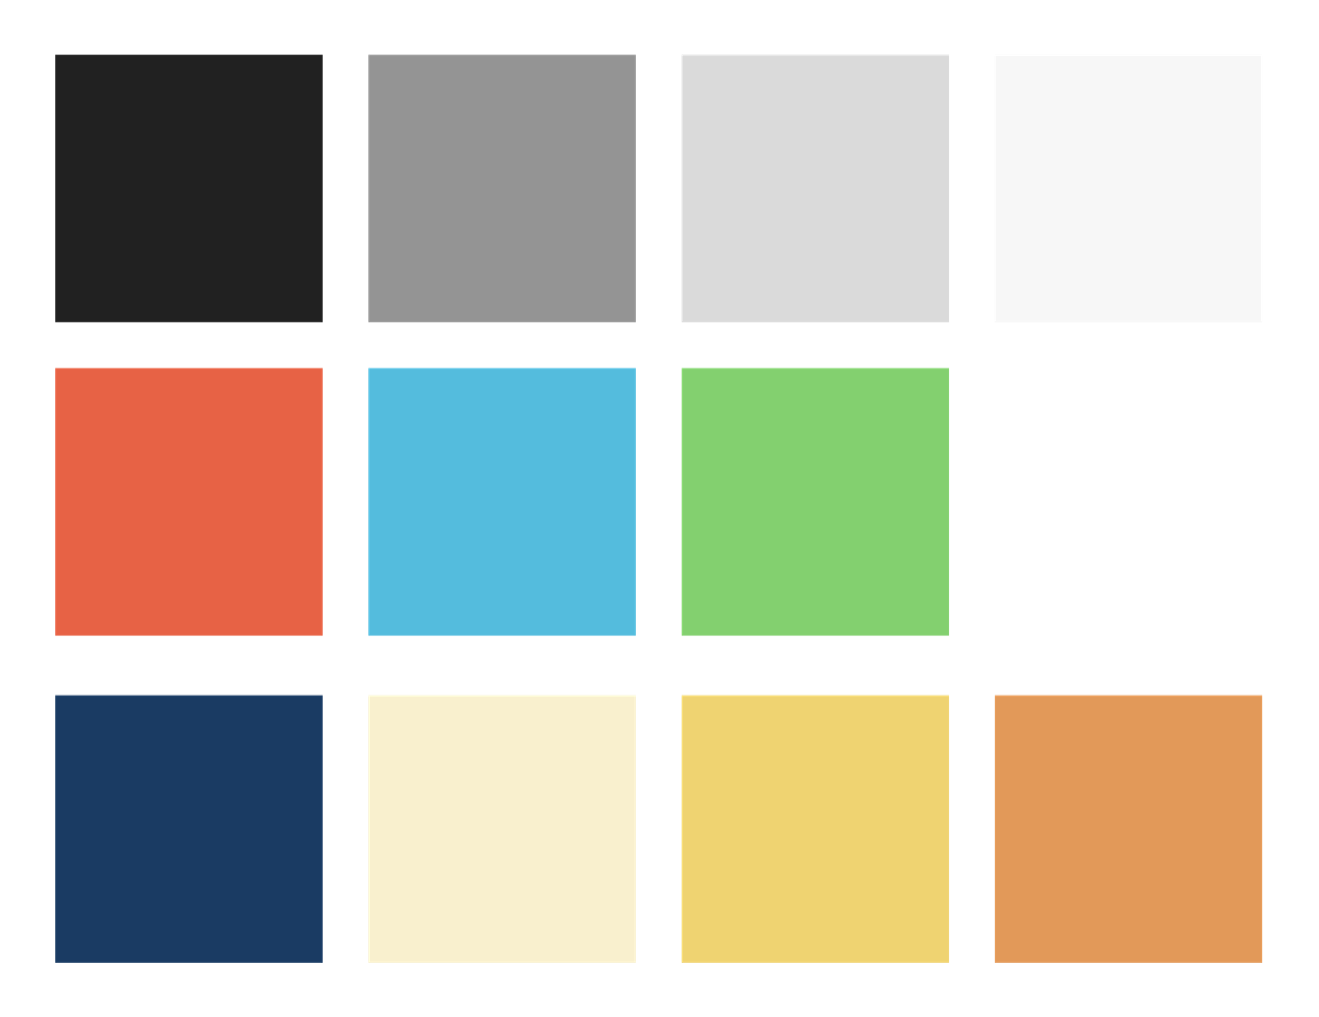
\includegraphics[width=\linewidth/2]{images/app/colors.png}
    \caption*{Source: Author}
    \label{fig:falealgumacoisa-color-scheme}
\end{figure}

\subsubsection{Web app}

To allow easier access to the voice recording app, a web-based application will be developed. This factor positively influences the capacity of the app to update over time, when compared to an application developed in a native environment. It also enables users over mobile and desktop to access the same application, and although the layout may have to be redesigned, most logic is reused.

\subsubsection{Mobile First}

The design will use a mobile first approach, to ensure the user flow will be optimized when he is using a mobile device. The desktop flow will be designed and developed afterwards.

\subsubsection{Splash Screen}

As the user first enter the application, a splash screen will be shown to welcome him (mobile version in figure \ref{fig:falealgumacoisa-splash-page-design}). It contains the logo and an animation to draw the user's attention. After the animation, the home will be shown.

\begin{figure}[ht]
    \centering
    \caption{Fale Alguma Coisa Splash Page design}
    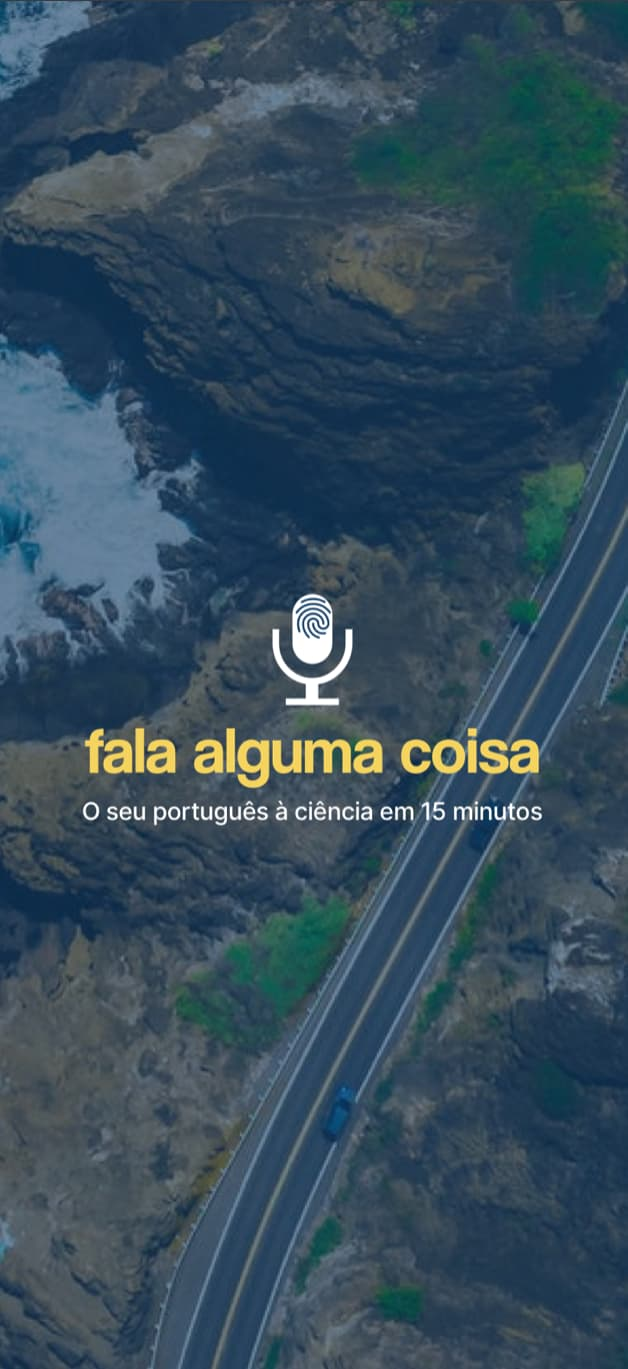
\includegraphics[width=\linewidth/2]{images/app/m-splash.jpg}
    \caption*{Source: Author}
    \label{fig:falealgumacoisa-splash-page-design}
\end{figure}

\subsubsection{Homepage}

After the splash animation, the homepage is shown. The mobile version can be seen below in figure \ref{fig:falealgumacoisa-home-page-design}. In this page, the call to action to start the recording is highlighted by the button at the center of the page, with text describing the project right below it. The login page is accessible through the link in the right upper corner. These few elements are placed to encourage the user to click on the recording, if he is a new user.

\begin{figure}[ht]
    \centering
    \caption{Fale Alguma Coisa Home Page design}
    \frame{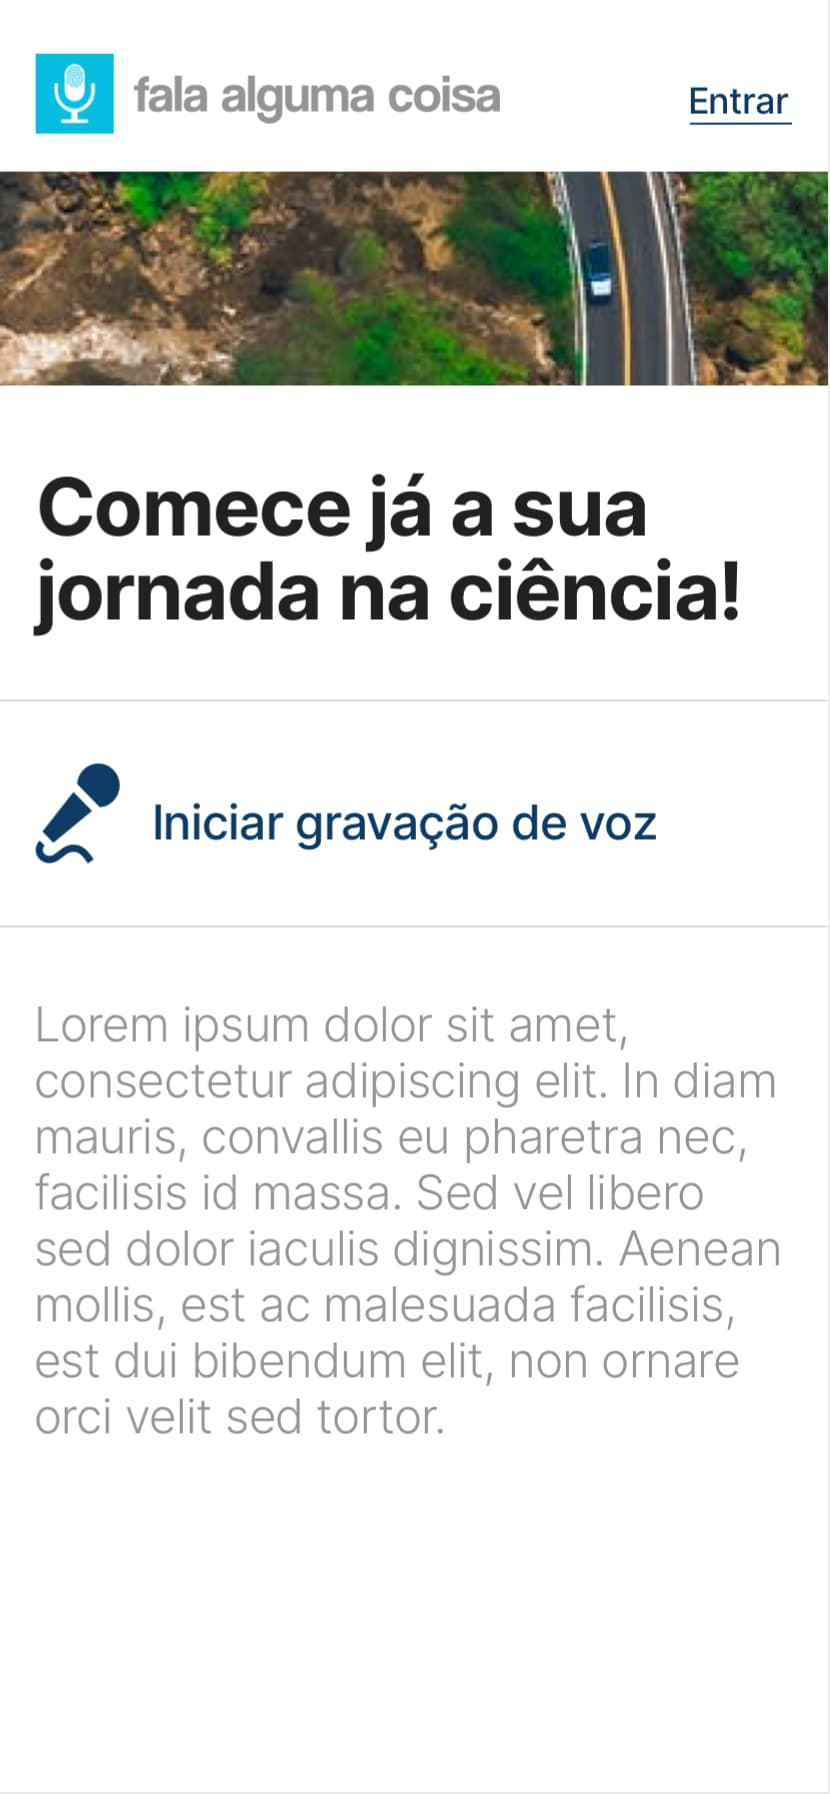
\includegraphics[width=\linewidth/2]{images/app/m-home.jpg}}
    \caption*{Source: Author}
    \label{fig:falealgumacoisa-home-page-design}
\end{figure}

\subsubsection{Recording}

This page represents the core functionality of the website, allowing the user to record phrases with his voice. The recording is done through groups of phrases, called a theme, and is illustrated by the image \ref{fig:falealgumacoisa-recording-page-design} at the bottom. The main elements of the page are (1) the phrase highlighted in a rectangular box at the center of the page, and (2) the red recording button at the bottom.

\begin{figure}[ht]
    \centering
    \caption{Fale Alguma Coisa Recording Page design}
    \frame{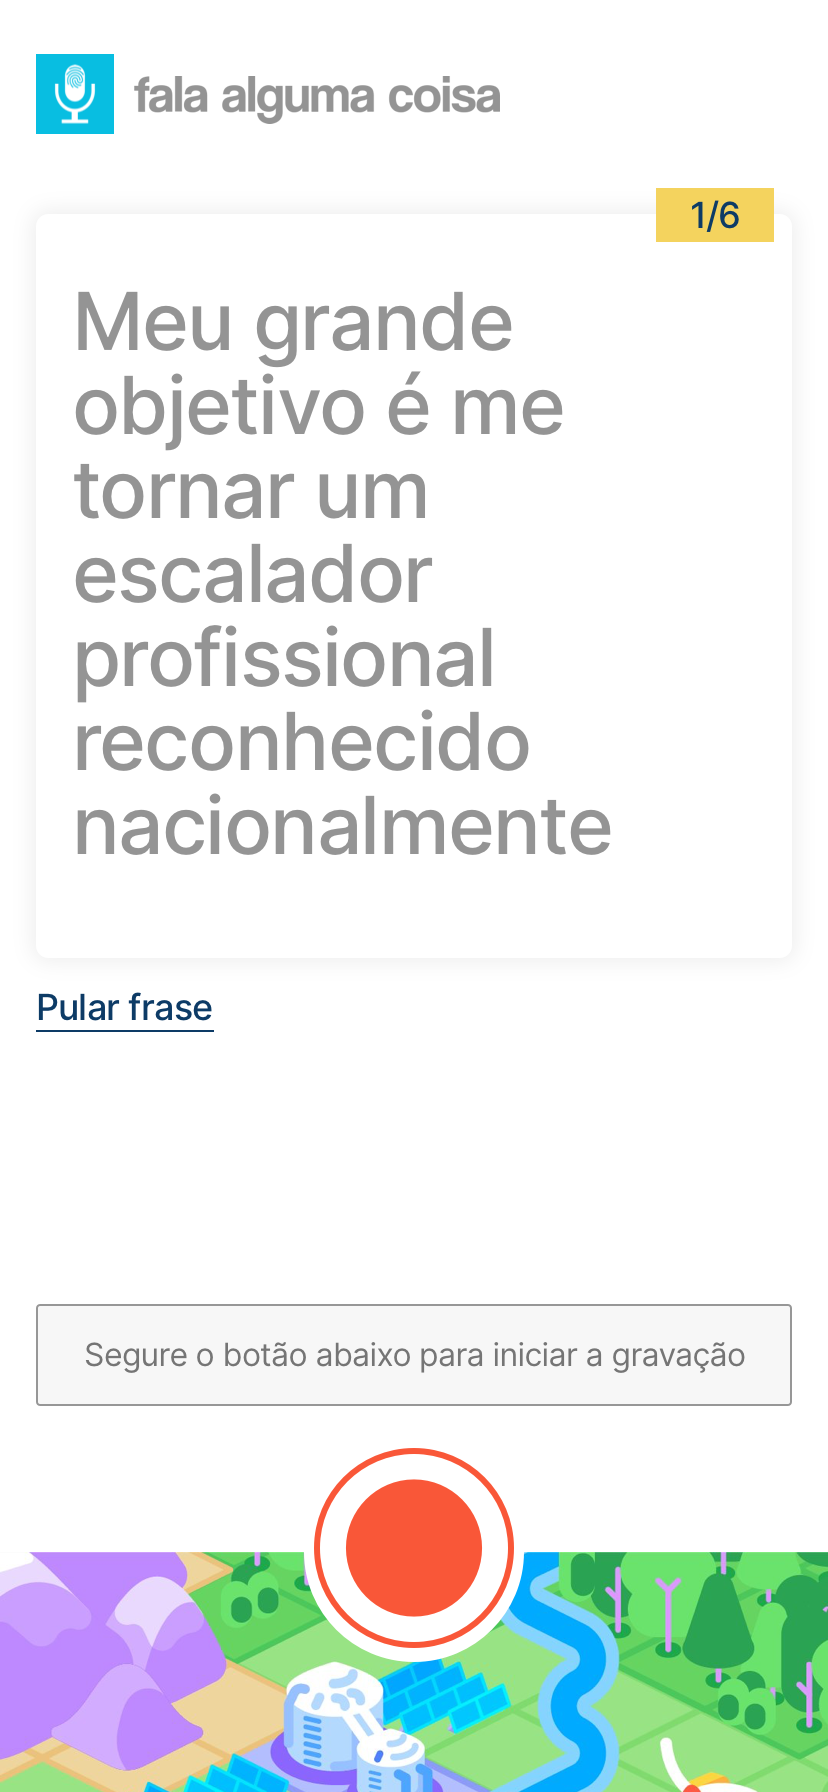
\includegraphics[width=\linewidth/2]{images/app/recording/Journey_1.0.png}}
    \caption*{Source: Author}
    \label{fig:falealgumacoisa-recording-page-design}
\end{figure}

\subsubsection{Dashboard}

When an unauthenticated user finishes recording its first theme, or when a user logs in, they are able to select from a list of themes to record. In this dashboard seen in figure \ref{fig:falealgumacoisa-dashboard-page-design}, they are also shown the number of points accumulated by the usage of the app, as well as able to open a menu and notification page.

\begin{figure}[ht]
    \centering
    \caption{Fale Alguma Coisa Dashboard Page design}
    \frame{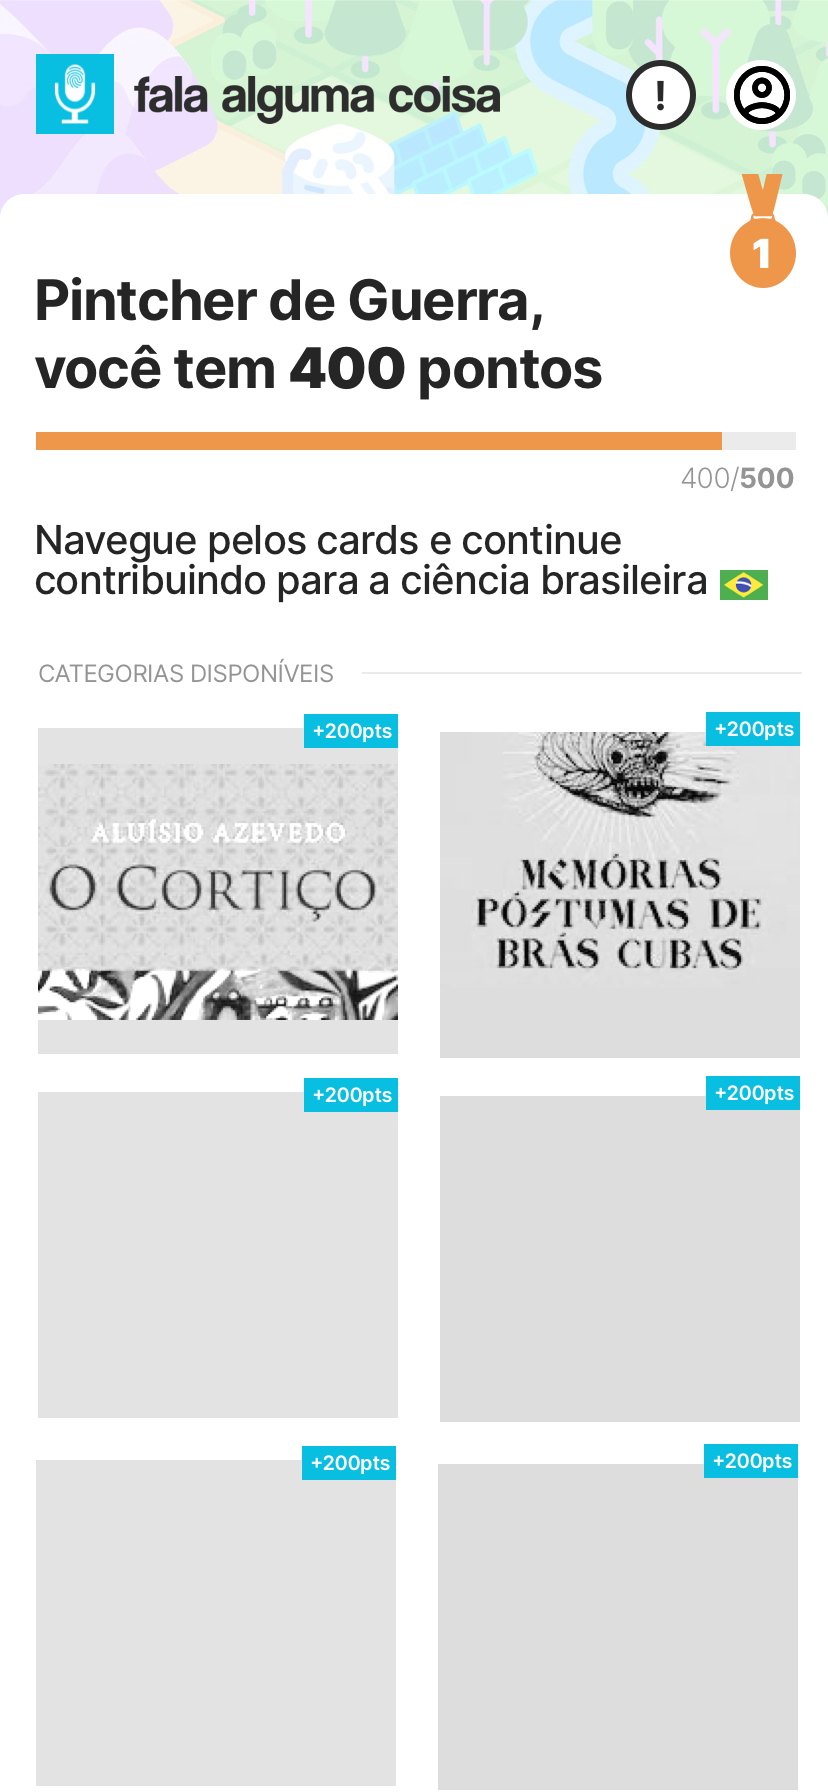
\includegraphics[width=\linewidth/2]{images/app/dashboard/Dashboard.png}}
    \caption*{Source: Author}
    \label{fig:falealgumacoisa-dashboard-page-design}
\end{figure}

\subsubsection{Leaderboard}

The leaderboard has two views: a list of the top ranking users (figure \ref{fig:falealgumacoisa-leaderboard-page-design-general}) and a list of friend rankings (figure \ref{fig:falealgumacoisa-leaderboard-page-design-friend}). They provide a way for users to compare their contributions, thus promoting competition. A social part is also included throughout the option to add friends.

\begin{figure}[ht]
    \centering
    \caption{Fale Alguma Coisa Leaderboard Page designs}
    \begin{subfigure}{.5\textwidth}
      \centering
      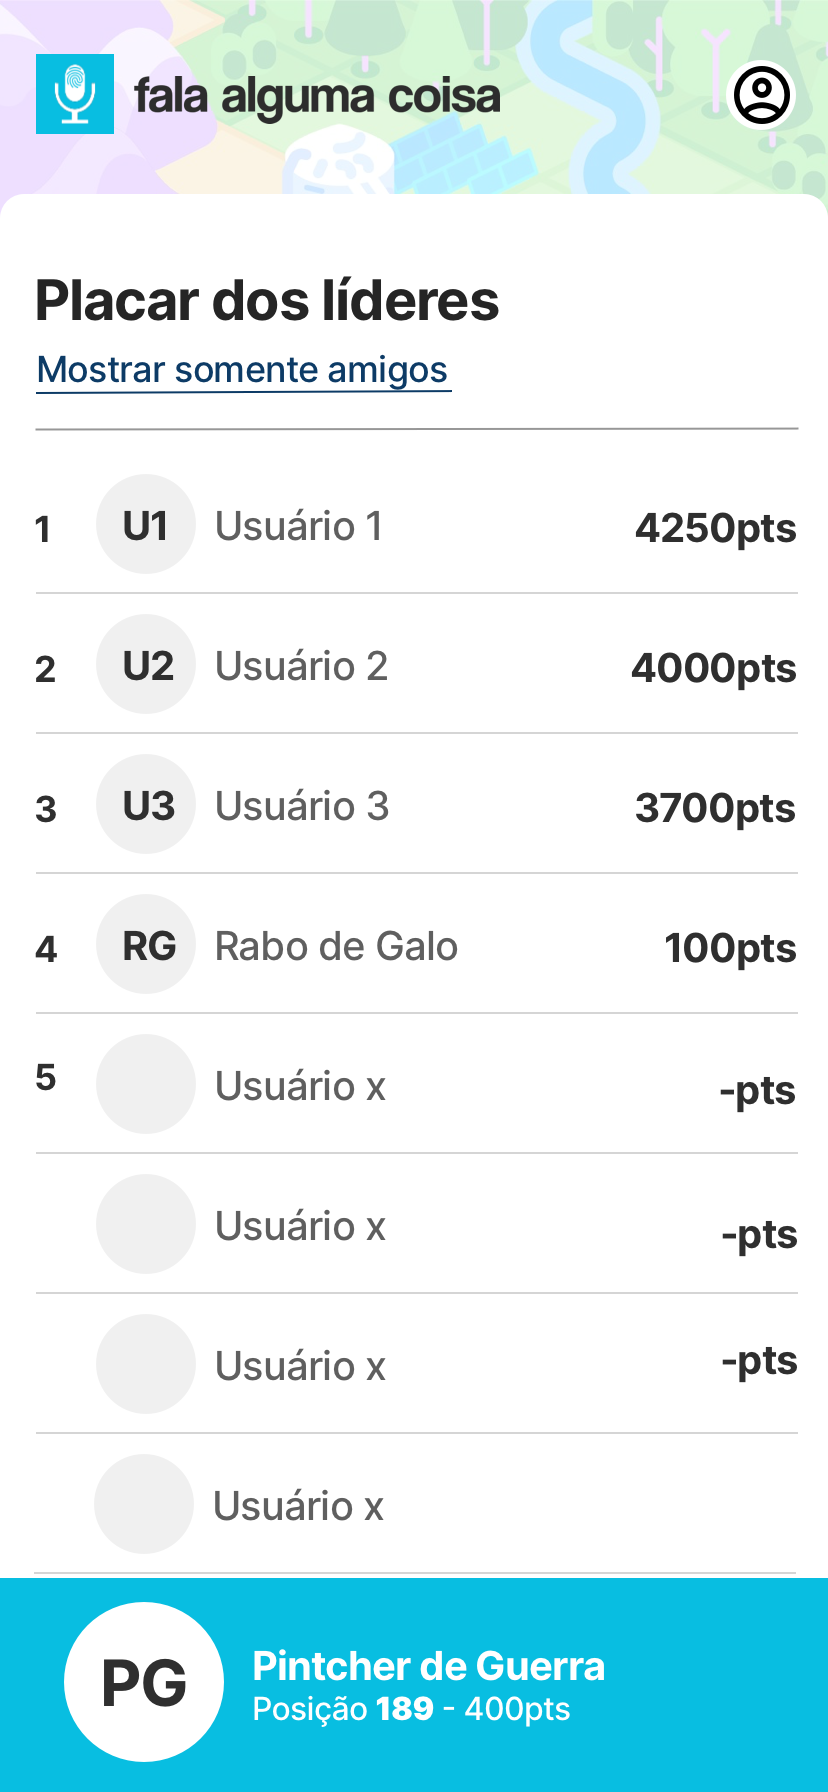
\includegraphics[width=.9\linewidth]{images/app/leaderboard/GeneralRanking.png}
      \caption{General Leaderboard}
      \label{fig:falealgumacoisa-leaderboard-page-design-general}
    \end{subfigure}%
    \begin{subfigure}{.5\textwidth}
      \centering
      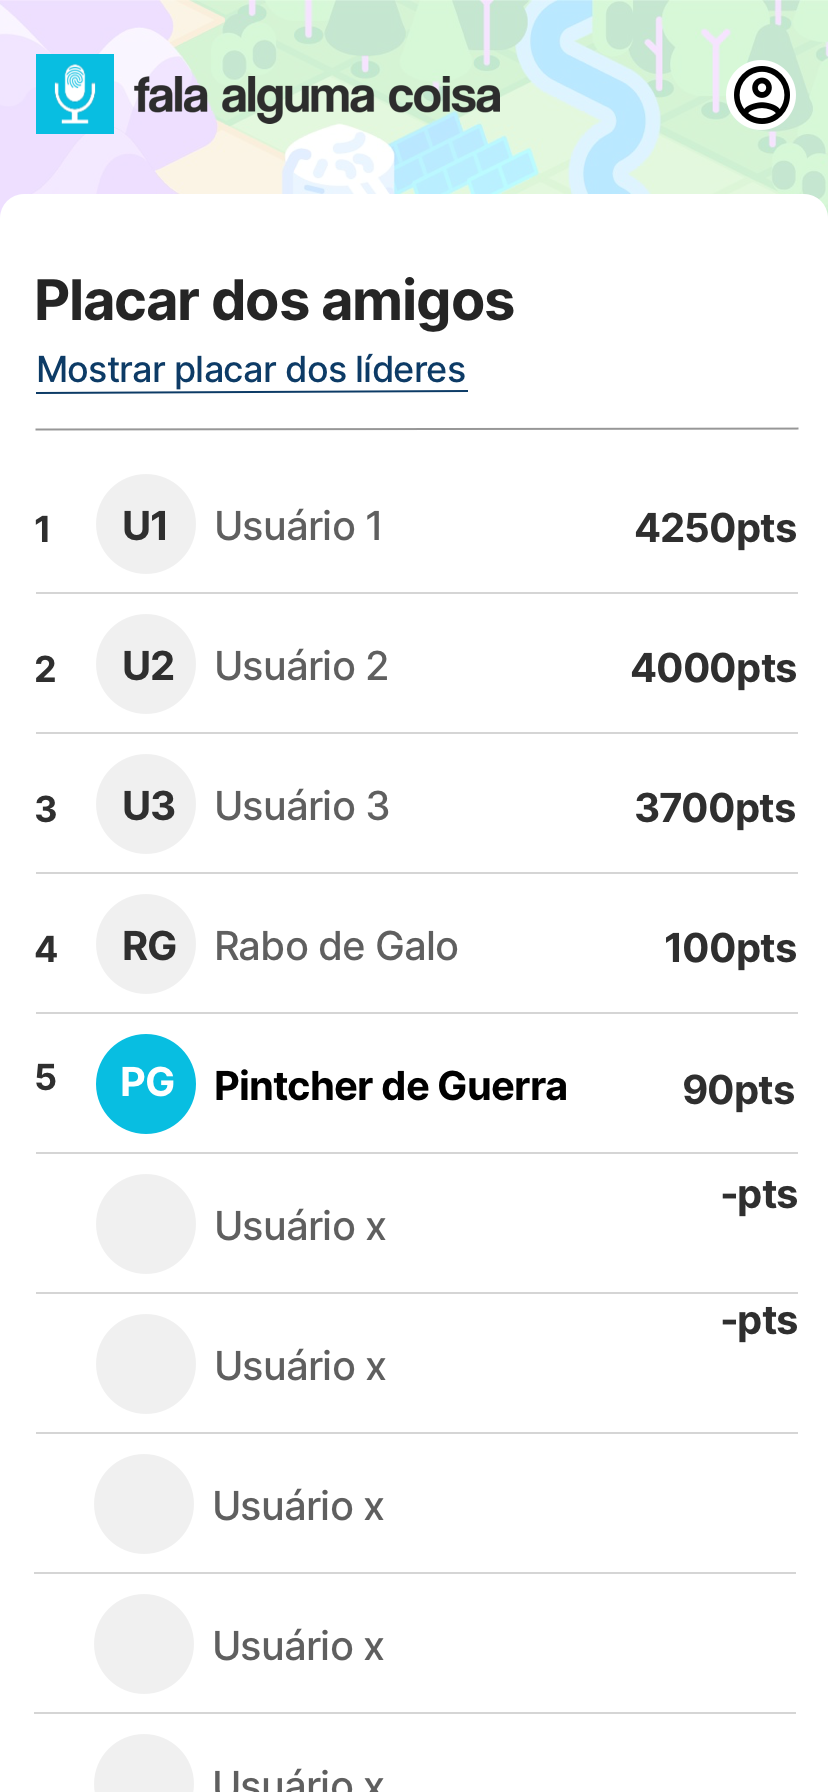
\includegraphics[width=.9\linewidth]{images/app/leaderboard/FriendsRanking.png}
      \caption{Friends Leaderboard}
      \label{fig:falealgumacoisa-leaderboard-page-design-friend}
    \end{subfigure}
    \caption*{Source: Author}
    \label{fig:falealgumacoisa-leaderboard-page-design}
\end{figure}

\subsubsection{Login and Registration}

The login and registration pages include essential features to the application: the ability to identify the user and maintain a history of recordings.

\begin{figure}[ht]
    \centering
    \caption{Fale Alguma Coisa Login and Registration Page designs}
    \begin{subfigure}{.5\textwidth}
      \centering
      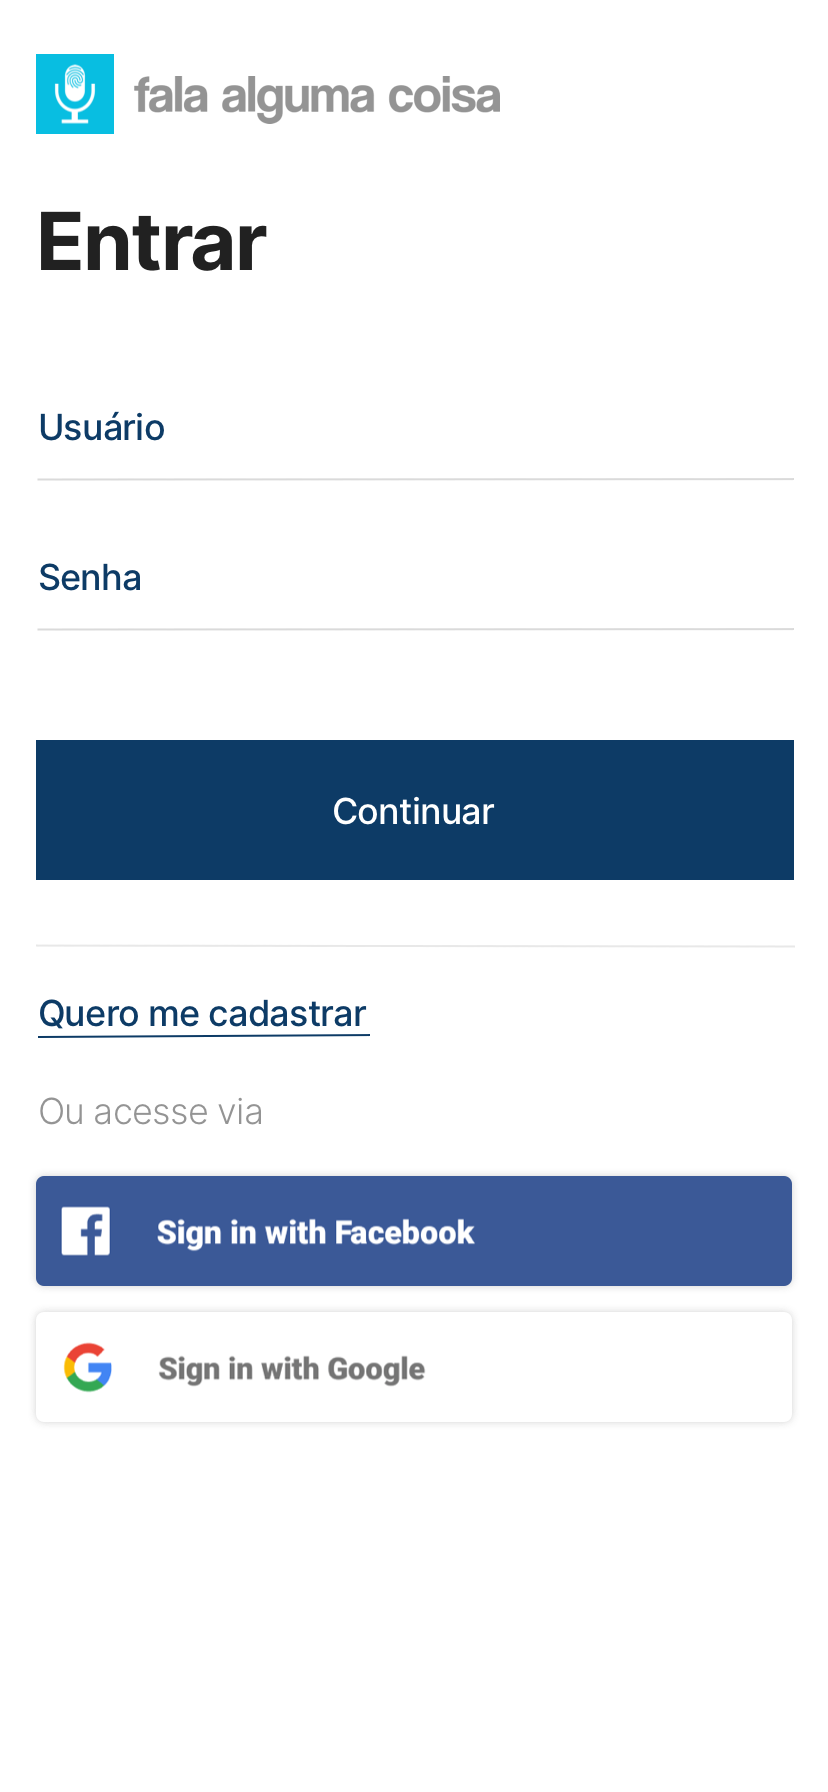
\includegraphics[width=.9\linewidth]{images/app/login/Login1.png}
      \caption{Login Page}
      \label{fig:falealgumacoisa-login-page-design}
    \end{subfigure}%
    \begin{subfigure}{.5\textwidth}
      \centering
      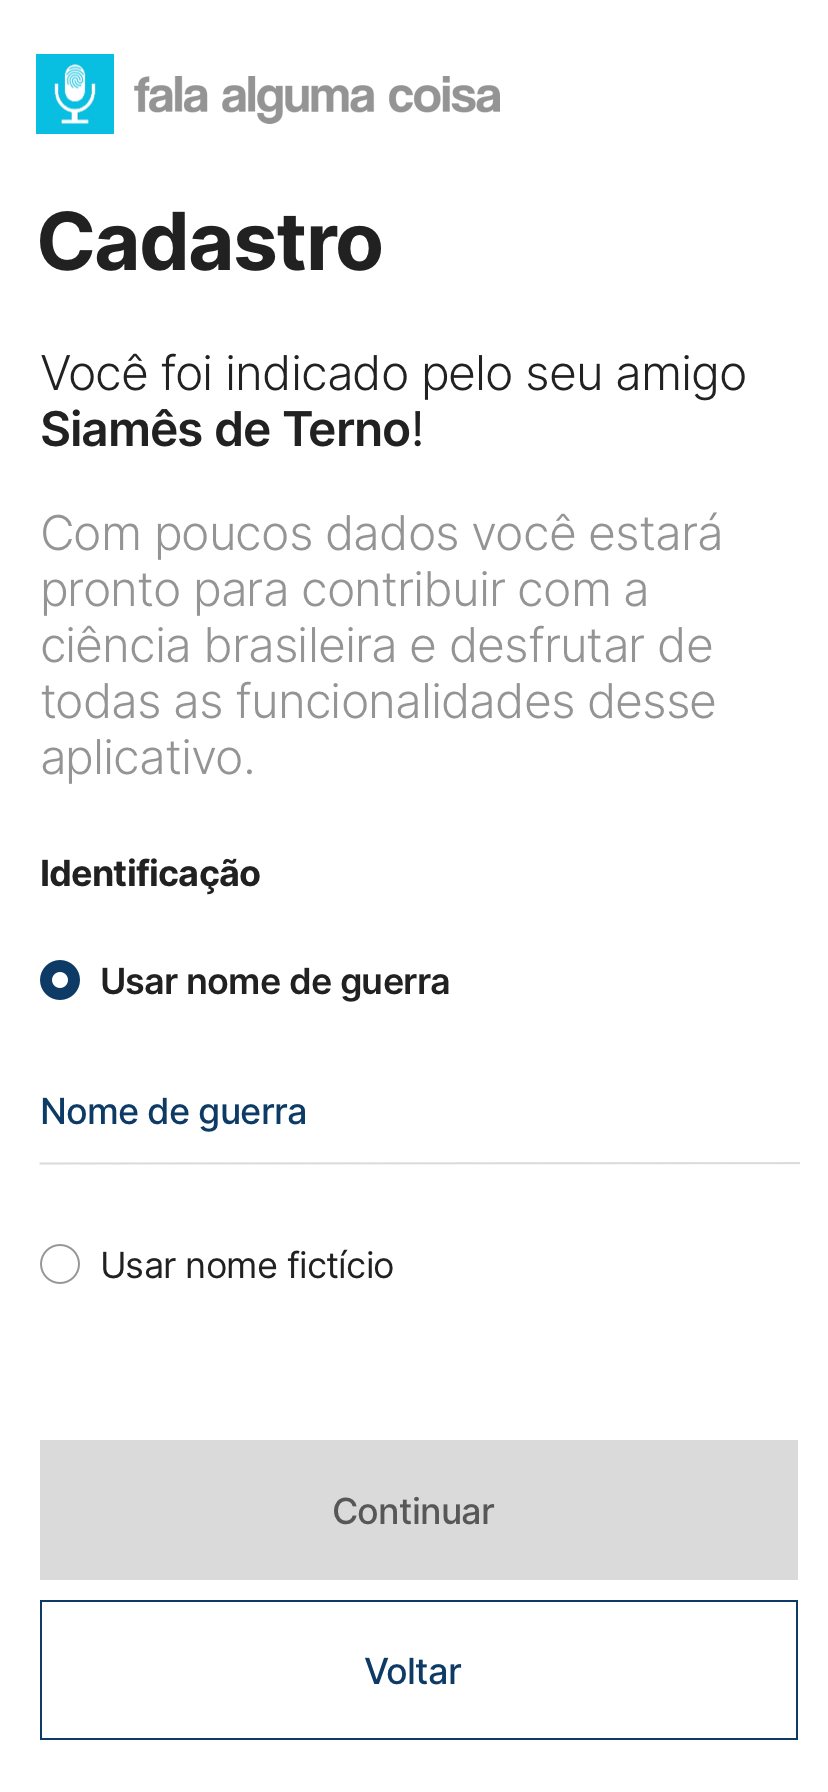
\includegraphics[width=.9\linewidth]{images/app/register/Register1.0.png}
      \caption{Registration Page}
      \label{fig:falealgumacoisa-registration-page-design}
    \end{subfigure}
    \caption*{Source: Author}
    \label{fig:falealgumacoisa-login-page-design}
\end{figure}

\subsubsection{Delete User}

If necessary, the user should be able to delete its user data, while still contributing his voice to the speech corpus. The following pages include the design of the layout for this deletion flow.

\begin{figure}[ht]
    \centering
    \caption{Fale Alguma Coisa Delete User Data Page design}
    \frame{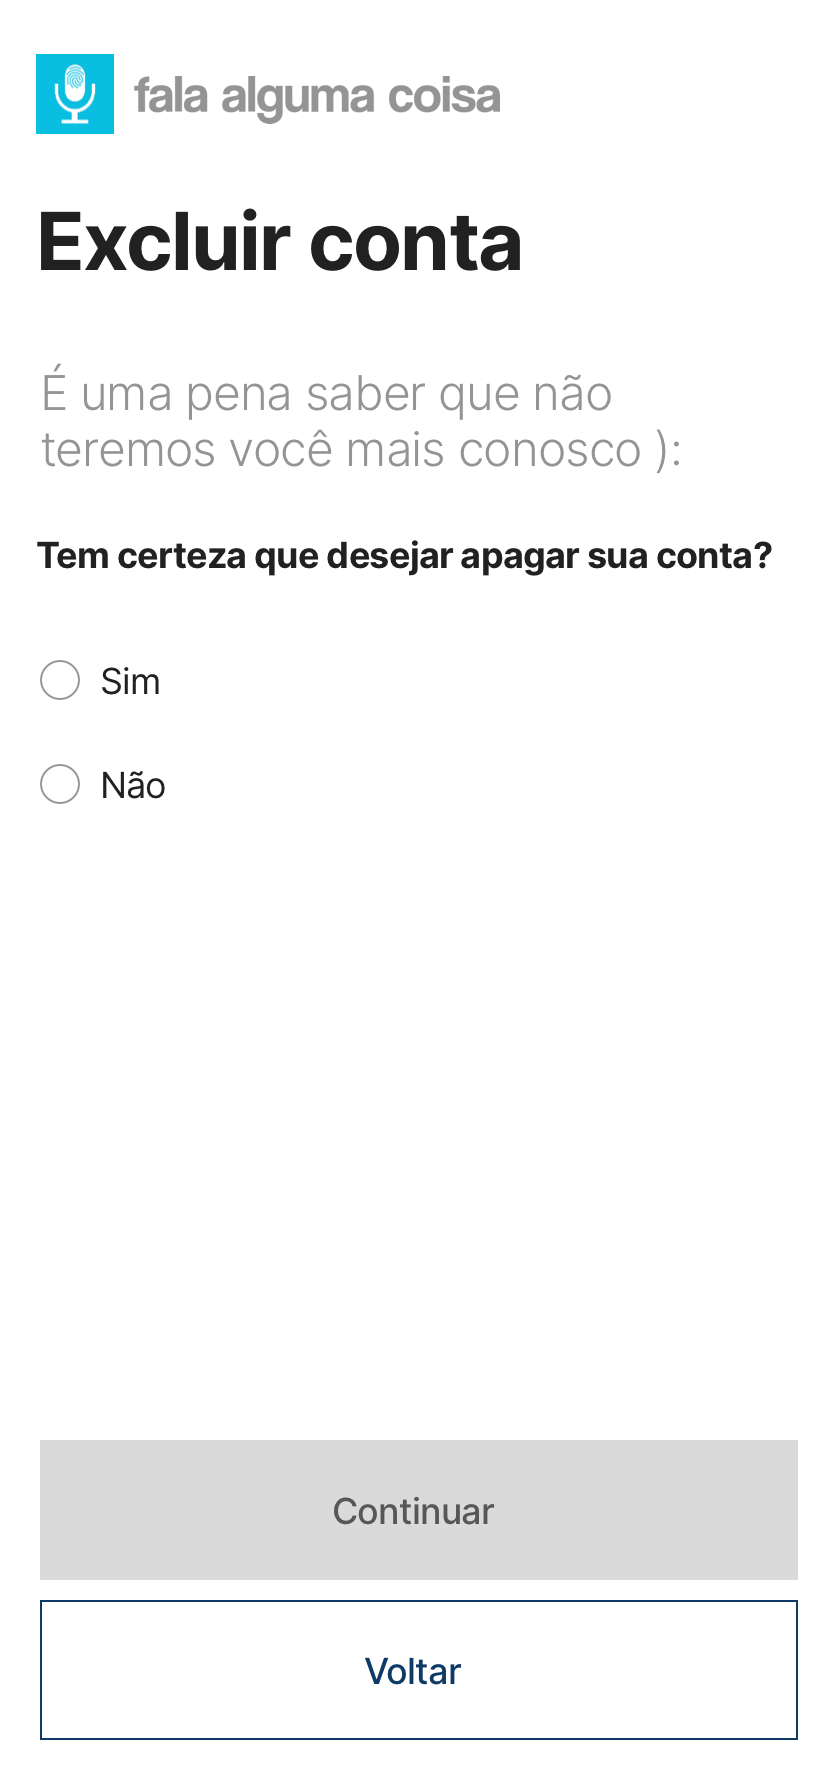
\includegraphics[width=\linewidth/2]{images/app/delete-user/FinishAccount1.0.png}}
    \caption*{Source: Author}
    \label{fig:falealgumacoisa-delete-user-data-page-design}
\end{figure}

\subsection{Development}

This section details the development process of the Fale Alguma Coisa app.

\subsubsection{Tools Selection}

To develop the application, a selection of tools was made. The table \ref{tab:tools-selection} details the selected tools and explains each choice.

\begin{table}[h]
    \centering
    \begin{tabular}{|c|c|c|}
        \hline Category & Selection & Explanation \\
        \hline Design & Zeplin & Easy sharing  \\ 
        \hline Desig &  & access \\ 
        \hline Galaxy Zoo & access & access \\ 
        \hline Christmas Audubom Birdwatch & access & access \\ \hline 
    \end{tabular}
    \caption{Contribution for online citizen science projects}
    \label{tab:cs-contributions}
\end{table}


\section{General Public Submission}
\label{sec:proposal-public-submission}

\section{Data Analysis}
\label{sec:proposal-data-analysis}

\section{Data Publication}
\label{sec:proposal-data-publication}
	\apendices 
\chapter{Ten principles of citizen science}
\label{app:ten-principles}

\begin{itemize}
    \item Citizen science projects actively involve citizens in scientific endeavour that generates new knowledge or understanding. 
    \subitem Citizens may act as contributors, collaborators or as project leaders and have a meaningful role in the project.
    \item Citizen science projects have a genuine science outcome. For example, answering a research question or informing conservation action, management decisions or environmental policy.
    \item Both the professional scientists and the citizen scientists benefit from taking part. Benefits may include the publication of research outputs, learning opportunities, personal enjoyment, social benefits, satisfaction through contributing to scientific evidence, for example, to address local, national and international issues, and through that, the potential to influence policy.
    \item Citizen scientists may, if they wish, participate in multiple stages of the scientific process. This may include developing the research question, designing the method, gathering and analysing data, and communicating the results.
    \item Citizen scientists receive feedback from the project. For example, how their data are being used and what the research, policy or societal outcomes are.
    \item Citizen science is considered a research approach like any other, with limitations and biases that should be considered and controlled for. However unlike traditional research approaches, citizen science provides opportunity for greater public engagement and democratisation of science.
    \item Citizen science project data and metadata are made publicly available and where possible, results are published in an open-access format. Data sharing may occur during or after the project, unless there are security or privacy concerns that prevent this.
    \item Citizen scientists are acknowledged in project results and publications.
    \item Citizen science programmes are evaluated for their scientific output, data quality, participant experience and wider societal or policy impact.
    \item The leaders of citizen science projects take into consideration legal and ethical issues surrounding copyright, intellectual property, data-sharing agreements, confidentiality, attribution and the environmental impact of any activities.
\end{itemize}

% 	% ----------------------------------------------------------


% 	% ----------------------------------------------------------
% 	% Prepara pdf para iniciar o bookmark na raiz
% 	% ----------------------------------------------------------
% 	\phantompart

% 	% ----------------------------------------------------------
% 	% Conclusão
% 	% ----------------------------------------------------------
% 	%\include{conclusao}
% 	% ----------------------------------------------------------

% 	% ----------------------------------------------------------
% 	% ELEMENTOS PÓS-TEXTUAIS
% 	% ----------------------------------------------------------
% 	\postextual
% 	% ----------------------------------------------------------

% 	% ----------------------------------------------------------
% 	% Referências bibliográficas
% 	% ----------------------------------------------------------
	\bibliography{referencias}

\end{document}